%%
%% Тема практики: <<Автоматизированная разработка программно-аппаратного комплекса
%% ''цифровые часы с будильником'' на базе микроконтроллера AVR семейства XMega>>
%%
\documentclass[russian,simple,utf8,pointsubsection,reduceheight=20mm]{eskdtext}
\usepackage[utf8]{inputenc}
\usepackage[russian]{babel}
\usepackage{ucs}
\usepackage[unicode]{hyperref}
\usepackage{multirow}
\usepackage{amstext}
\usepackage{amsmath}
\usepackage{listings}
\graphicspath{{/Users/zolkko/Projects/zolkko-alarm/doc/imgs/}}
\usepackage{longtable}
\usepackage{geometry}



\ESKDdepartment{}
\ESKDcompany{}
\ESKDclassCode{31 1398}
\ESKDdocName{Пояснительная записка}
\ESKDsignature{Автоматизированная разработка программно-аппаратного комплекса на базе микроконтроллера AVR семейства XMega}
\ESKDtitle{Отчёт по преддипломной практике}
\ESKDauthor{Анисимов~А.~Н.}
\ESKDtitleApprovedBy{Руководитель}{Барабанов~В.~Ф.}
\ESKDtitleAgreedBy{Руководитель}{Барабанов~В.~Ф.}
\ESKDtitleDesignedBy{студент группы ВМ-072}{Анисимов А.Н.}

%% первая страница и титульный лист без рамок и кастомный формат
\ESKDdefaultTitleStyle{empty}
\ESKDdefaultFirstStyle{empty}
\ESKDdefaultStyle{empty}

%% Уменьшаю размер шрифта колонки №1 основной надписи, так что бы эта
%% "умная" дура всё таки влезла в рамку
\renewcommand{\ESKDfontVIIsize}{\fontsize{10pt}{12pt}}

%% пол умалчанию перечисления используют арабские цифры
\renewcommand{\theenumi}{\arabic{enumi}}

%% Сказали, что в перечислених ни каких булетов не должно быть
\renewcommand{\labelitemi}{}
\renewcommand{\labelitemii}{}
\renewcommand{\labelitemiii}{}
\renewcommand{\labelitemiv}{}

%% Главные заголовки центрируються
\renewcommand{\ESKDsectionAlign}{\ESKDsectAlignCenter}
\renewcommand{\ESKDsectionStyle}{\normalfont\MakeUppercase}
\renewcommand{\ESKDsubsectionStyle}{\normalfont}
\renewcommand{\ESKDsubsubsectionStyle}{\normalfont}

%% \renewcommand{\bibname}{Test}


\geometry{left=20mm}
\geometry{right=20mm}
\setlength{\footskip}{0mm}


\begin{document}
\pagestyle{plain}
\thispagestyle{empty}
\begin{center}
Федеральное агентство по образованию \\*
ГОСУДАРСТВЕНОЕ ОБРАЗОВАТЕЛЬНОЕ УЧРЕЖДЕНИЕ \\*
ВЫСШЕГО ПРОФЕССИОНАЛЬНОГО ОБРАЗОВАНИЯ \\*
<<ВОРОНЕЖСКИЙ ГОСУДАРСТВЕННЫЙ ТЕХНИЧЕСКИЙ УНИВЕРСИТЕТ>> \\
\end{center}
\begin{center}
Факультет  автоматики и электромеханики \\
\end{center}
\begin{center}
Кафедра автоматизированных и вычислительных систем \\
\end{center}

\begin{center}
Специальность 230101 <<Вычислительные машины, комплексы, системы и сети>>
\end{center}

\vspace{1em}

\begin{center}
ОТЧЁТ \\*
ПО ПРЕДДИПЛОМНОЙ ПРАКТИКЕ \\*
Тема практики: <<Автоматизированная разработка программно-аппаратного комплекса
''цифровые часы с будильником'' на базе микроконтроллера AVR семейства XMega>>
\end{center}

\vspace{1em}

\begin{tabular}{p{12em}p{5em}@{}p{5em}@{}r@{}r}
Выполнил студент группы & \hrulefill{} ВМ-072 & \hrulefill{}  & \hrulefill{} А.Н. Анисимов \\
 &  \small{Группа}  & \small{Подпись} &\small{Инициалы, фамилия} \\
& & & \\
\multirow{2}{12em}{Руководитель практики\newline{} от кафедры АВС} & \hrulefill{} & \hrulefill{} & \hrulefill{} О. Я. Кравец \\
 & \small{Подпись}  & \small{Дата} & \small{Инициалы, фамилия} \\
 & & & \\
\multirow{2}{12em}{Руководитель дипломного  проекта} & \hrulefill{} & \hrulefill{} & \hrulefill{} А. В. Барабанов \\
 & \small{Подпись}  & \small{Дата} & \small{Инициалы, фамилия} \\
& & & \\
\multirow{2}{12em}{Консультант дипломного проекта} & \hrulefill{} & \hrulefill{} & \hrulefill{} В.Ф. Барабанов \\
 & \small{Подпись}  & \small{Дата} & \small{Инициалы, фамилия} \\
& & & \\
\multirow{2}{12em}{Руководитель по экономической части} & \hrulefill{} & \hrulefill{} & \hrulefill{} Т.С. Наролина \\
 & \small{Подпись}  & \small{Дата} & \small{Инициалы, фамилия} \\
& & & \\
Защищена \hrulefill{} &  & Оценка \hrulefill{} & \hrulefill{} 
\end{tabular}

\vspace{1.5em}

\begin{center}
г. Воронеж \\*
2011 г.
\end{center}

\newpage

\setlength{\footskip}{10mm}

\renewcommand{\contentsname}{СОДЕРЖАНИЕ}


\begin{center}
\MakeUppercase{ЗАМЕЧАНИЯ РУКОВОДИТЕЛЯ}
\end{center}
\newpage

%% Постановка задачи
\section{Постановка задачи}
\begin{par}
Спроектировать и разработать устройство позволяющее в заданные моменты времени выдавать сигнал
звукового оповещения, производить индикацию текущего времени, а так же прозводить его синхронизацию
с удалённым сервером используя вычислительную сеть стандарта 802.3 Ethernet.
\end{par}

\begin{par}
Центральный вычислительный модуль устройства должен быть выполнен на микроконтроллере AVR компании
Atmel семейства XMega.
\end{par}

\begin{par}
Не смотря на то, что реализация подобного устройства на ПЛИС имеет ряд преимуществ по
сравнению с реализацией на основе микроконтроллеров, а именно более высокая скорость
работы и более низкое потребление энергии, новое семейство 8-битных микроконтроллеров
AVR переносит микроконтроллерные устройства на новый уровень системных характеристик,
которые в сочетации с более низкой стоимостью самих микроконтроллеров и иструментария
разработчика, делает их адекватным выбором при проектировании систем. Микроконтроллеры
AVR семейства XMega интегрируют в себе устройства ввода-вывода с улучшенными характеристиками,
более низкую потребляемую мощьность за счёт применения в них новой технологии picoPower.
Новая система обработки событий Event System, обеспечивает независимую от ЦПУ
быстродействующую передачу данных между внутренними переферийными устройствами 4-канального
контроллера ПДП, улучьшающего характеристики микроконтроллера. Микроконтроллеры имеют
быстродействующие 12-битнее модули АЦП и ЦАП. И ускоритель криптографических алгоритмов AES и DES.
Каждое перечисленное нововведение в семействе XMega микроконтроллеров AVR, позволит
в более сжатые сроки, а следовательно и с меньшими финансовыми затратами реализовать
целевое устройство, при этом отставание в производительности и потребляемой мощьности
становиться не значительным для данного класса устройств.
\end{par}

\begin{par}
Необходимо в качестве устройств ввода и вывода использовать один модуль сенсорного экрана
для уменьшения рабочей поверхности изделия.
\end{par}

\begin{par}
В качестве устройства взаимодействия с удалённым сетевым сервисом времени необходимо использовать
контроллер фирмы Micro Chip enc28j60. Применени этого контроллера позволит устройству производить
синхронизацию текущего времени по протоколу SNTP.
\end{par}

\begin{par}
Необходимо споектировать и разработать:
    \begin{itemize}
        \item{}Принципиальную электрическую схему;
        \item{}печатную плату.
    \end{itemize}
\end{par}

\begin{par}
Необходимо разработать на языке высокого уровня С++  программу управления устройва:
\begin{itemize}
    \item{} Модуль учёта текущего времени;
    \item{} модуль индикации текущего времени, выводящий информацию о текущем времени на ЖК-дисплее;
    \item{} модуль пользовательского ввода с сенсорного экрана, обеспечивающий первоначальную
            конфигурацию устройства, и установку времени срабатывания звукового сигнала;
    \item{} модуль воспроизведения звукового сигнала с внешней энергонезависимой памяти;
    \item{} модуль синхронизации текущего времени с удалённым SNTP сервисом.
\end{itemize}
\end{par}
\newpage{}

\newpage{}

%% Реферат
\begin{center}\MakeUppercase{Реферат}\end{center}
\addcontentsline{toc}{section}{Реферат}

Пояснительная записка \ESKDtotal{page} с., \ESKDtotal{figure} рисунков, \ESKDtotal{table} таблиц, \ESKDtotal{bibitem} источников.
Ключевые слова --- AVR, XMega, автоматизированная разработка.


Объект исследования или разработки --- создание КП <<Универсальная система терморегулирования
 на базе микроконтроллера AVR семейства XMega>>.

\newpage{}










\newpage{}


%% В ВГТУ по какой-то причине не считаются с существованием ЕСКД
%\ESKDthisStyle{formI}
%\setcounter{page}{3}
\tableofcontents
\newpage{}

%% Введение
%!TEX root = /Users/zolkko/Projects/zolkko-alarm/doc/main.tex
\section*{Введение}
\addcontentsline{toc}{section}{Введение}
\begin{par}
На сегодняшний день при проектировании систем промышленной автоматизации и устройств
бытового применения, перед проектировщиками и разработчиками встают вопросы не только технического
характера, но и вопросы экономической целесообразности применения тех или иных решений.
То есть при их решении необходимо учитывать не только системные характеристики применяемых для
реализации конечных устройств технологий, но и искать компромис с их стоимостью. При этом
на конечную стоимость изделия будут влиять цена применённых схемотехнических решений,
время затраченное на проектирование и реализацию устройства, цена применяемых средства автоматизации
и цена специалистов проектировщиков и разработчиков.
\end{par}

\begin{par}
Немаловажным при проектировании устройств является учёт стремления
современной европейской культуры не только к открытым, но и полностью свободным системам,
зачастую обладающим более качественными системными и
потребительскими характеристиками и способствующими общему\\*
научно-техническому прогрессу \cite{lessing}.
\end{par}


В дипломном проекте рассмотрены современные методы и средства проектирования и разработки
программно-аппаратным комплексов на базе микроконтроллеров AVR компании Ateml. При этом
в процессе проектирования и разработки отдавалось предпочтение именно свободному или
доступному по цене программному и аппаратному обеспечению. В качестве примера разрабатывался
программно-аппаратный комплекс <<Универсальная система терморегулирования на базе
микроконтроллера AVR cемейства XMega>>. Таким образом в процессе выполнения дипломного проекта
стало возможным проведение анализа пригодности для практического применения свободного,
бесплатного и доступного по цене программного и аппаратного обеспечения для целей промышленного
производства.

Программный код написанный в процессе выполнения дипломного проекта использует большинство
внешней периферии микроконтроллера. Таким образом, сформированный программный код и электрическая
принципиальная схема, позволяют оценить преимущества и недостатки использования
микроконтроллеров AVR семейства XMega.

\newpage{}



%% Обзор САПР
%!TEX root = /Users/zolkko/Projects/zolkko-alarm/doc/main.tex
\section{Анализ современных систем автоматизированного проектирования про\-гра\-ммно\--аппа\-ра\-тных микроконтроллерных комплексов}

\subsection{Общие сведения о САПР}
\begin{par}
САПР --- Система автоматизированного проектирования --- автоматизированная система, реализующая
информационную технологию выполнения функций проектирования, представляет собой
организационно-техническую систему, предназначенную для автоматизации процесса проектирования,
состоящую из персонала и комплекса технических, программных и других средств
автоматизации его деятельности.
\end{par}

\begin{par}
На некотором этапе своего развития системы проектирования претерпели качественное изменение.
Оно было связано с тем, что САПР из набора каким-то образом связанных между собой прикладных
программ начали превращаться в мобильные и стройно организованные системы, способные к
настройке на особенности предметной области и на требования конечного пользователя,
допускающие расширение функциональных возможностей за счёт сравнительно несложного подключения
новых прикладных программных модулей и обеспечивающих поддержку групповой разработки сложных схем
коллективом проектировщиков.
\end{par}

\begin{par}
Особенное значение САПР приобрели в микроэлектронике, поскольку современная радиоэлектронная аппаратура базируется на применении сверхбольших
интегральных схем, разработка которых без применения САПР невозможна или крайне затруднительна.
\end{par}

\begin{par}
Специализированные САПР для разработки электронных устройств и печатных плат получили название
Electronic Design Automation - EDA, автоматизация проектирования электронных приборов.
Комплексы такого типа зачастую позволяют создавать принципиальные электрические схемы схемы с
помощью графического интерфейса, создавать и модифицировать  базу радиоэлектронных компонентов,
проверять целостность сигналов на ней и проводить аналоговое и цифровое моделирование
разрабатываемого устройства ещё на этапе проектирования.
\end{par}


\subsubsection{Обзор Electric VLSI}
\begin{par}
Electric VLSI --- cистема автоматизированного проектирования сверхбольших интегральных схем, используемая для разработки электрических схем и проектирования
топологии печатных плат и интегральных схем.
\end{par}
\begin{par}
Electric являлся open-source проектом, разработка
которого в течении многих лет поддерживалась\cite{electric} компанией Sun Microsystems,
а в настоящее время курируется компанией Oracle. \\*
Наиболее ценная встроенная в Electric возможность —-- это система привязок,
которая даёт возможность осуществлять проектирование сверху вниз с соблюдением целостности
всех соединений.
\end{par}

\subsubsection{Обзор Proteus VSM}
\begin{par}
Proteus VSM --- пакет программ для автоматизированного проектирования электронных схем.
    Разработка компании Labcenter Electronics.
\end{par}
\begin{par}
Proteus VSM сочитает в себе функциональность SPICE симуляции электронных цепей,
анимированные компоненты, модели микропроцессоров и средства симуляции сложных
микроконтроллерых решений. Это первая система сочетающая в себе все эти особенности
и позволяющая разработать и протестировать решение до создания прототипа устройства.
Такое тестирование осуществляется за счёт взаимодействия с отображаемыми и анимированными
виртуальными устройствами такими как свето-диоды, LCD, кнопки и переключатели.
При этом симуляция производится в режиме блиском к режиму реального времени.
Так производительности 1 ГГц Pentium III ЭВМ будет достаточно для симуляции работы
микропроцессора 8051 на частоте 12 МГц в режиме реального времени. Так же Proteus VSM
предоставляет экстенсивные средства отладки, включая точки останова, трассировку и вывод
значений  переменных микропрограмм как для машинных кодов, так и для языков высокого
уровня. Proteus VSM  включает несколько виртуальныхинструментов: осцилограф, логический
анализатор, генератор функций, генератор по шаблонам, виртуальный терминал, отладчики SPI
и I2C интерфейсов , а так же простые инструменты как вольтметр и амперметр, существенно
облегчающих анализ и отладку схемы.
\end{par}
\begin{par}
В дополнении к моделям микропроцессоров в Proteus VSM так же включена большая библиотека
стандартных пассивных и акивных моделей устройств.
\end{par}
\begin{par}
Пакет Proteus состоит из двух частей, двух подпрограмм: ISIS – программа синтеза и
моделирования непосредственно электронных схем и ARES – программа разработки печатных
плат.

\begin{figure}[h]
	\center{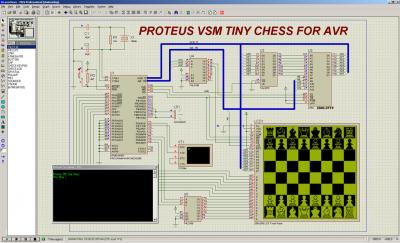
\includegraphics[bb=0 0 400 243, clip, scale=0.8]{proteus.png}}
	\caption{Главное окно программы Proteus ISIS}
	\label{img:proteus}
\end{figure}

\end{par}

\subsubsection{Обзор KiCAD}
\begin{par}
KiCad --- распространяемый по лицензии GNU General Public License программный
комплекс класса EDA с открытыми исходными текстами, предназначенный для разработки
электрических схем и печатных плат. \\*
Кроссплатформенность компонентов KiCad обеспечивается использованием библиотеки wxWidgets.
Поддерживаются операционные системы Linux, Windows NT 5.x, FreeBSD и Solaris.
\begin{figure}[h]
	\center{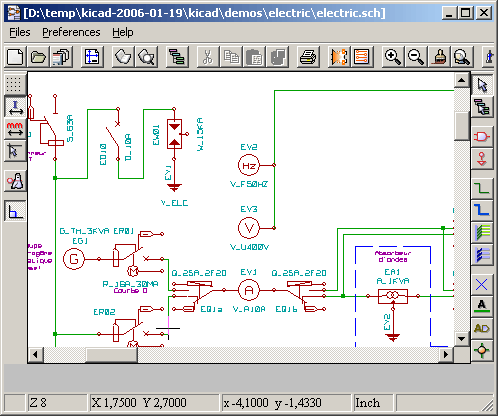
\includegraphics[bb=0 0 498 416, clip, scale=0.5]{kicad.png}}
	\caption{Главное окно программы KiCAD Eeschema}
	\label{img:kicad}
\end{figure}
\end{par}

\begin{par}
В состав KiCAD входят программы:
    \begin{itemize}
        \item{}kicad --— менеджер проектов;
        \item{}eeschema —-- редактор электрических схем (рис. \ref{img:kicad});
        \item{}встроенный редактор символов схем (библиотечных компонентов);
        \item{}pcbnew --— редактор печатных плат;
        \item{}встроенный редактор образов посадочных мест (библиотечных компонентов);
        \item{}3D Viewer --— 3D-просмотрщик печатных плат на базе OpenGL (часть pcbnew);
        \item{}gerbview --— просмотрщик файлов Gerber (фотошаблонов);
        \item{}cvpcb --— программа для выбора посадочных мест, соответствующих компонентам на схеме;
        \item{}wyoeditor --— текстовый редактор для просмотра отчетов.
    \end{itemize}
\end{par}


\subsubsection{Обзор gEDA}
\begin{par}
gEDA --- набор программного обеспечения для проектирования электронных устройств,
распространяемый по лицензии GPL. Включает в себя инструменты для редактирования
электрических схем, симуляции цифровых и аналоговых схем, трассировки печатных плат
и подготовки к производству. Проект изначально ориентирован на UNIX-совместимые
платформы, хотя некоторые программы, входящие в его состав, в настоящее время
портированы под ОС Windows\cite{geda}.
\end{par}
\begin{par}
В настоящее время пакет вполне пригоден для проектирования устройств среднего уровня
сложности и может быть полезен как студентам, любителям, так и профессиональным
разработчикам электронных устройств.
\end{par}
\begin{par}
За время существования проекта, к нему примкнуло несколько самостоятельных
узкоспециализированных проектов, которые теперь считаются частью gEDA, в
связи с чем оригинальный проект и его составные части стали называть
gEDA/gaf (gschem and friends) (рис. \ref{img:geda}).
\begin{figure}[h]
	\center{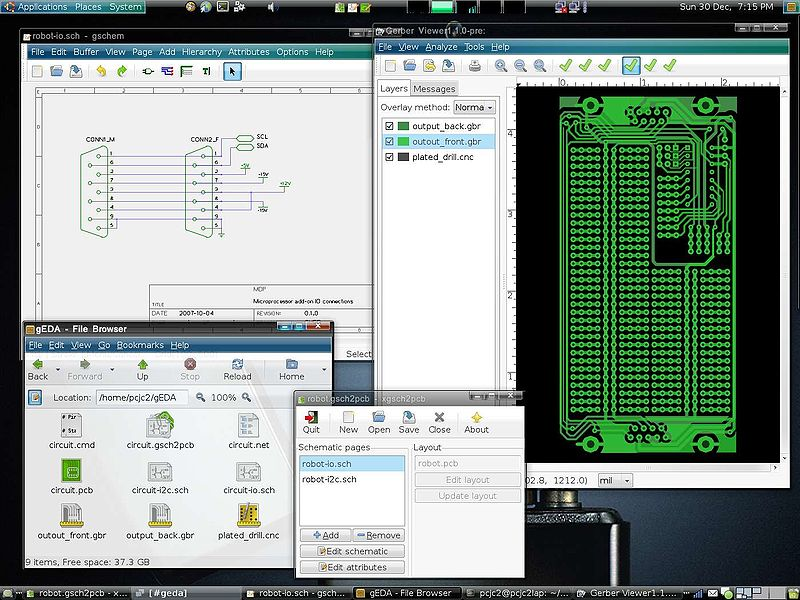
\includegraphics[bb=0 0 800 600, clip, scale=0.3]{geda.png}}
	\caption{gEDA}
	\label{img:geda}
\end{figure}
\end{par}

\subsubsection{Обзор Eagle EDA}
\begin{par}
EAGLE это лёгкий в использовании, но достаточной мощный EDA пакет, разрабатываемый немецкой компанией CadSoft.
В состам системы входят:
\begin{enumerate}
	\item{}Layout Editor --- пограмма для проектирования печатных плат (рис. \ref{img:eagle_brd}). 
		\begin{itemize}
			\item{}Максимальная рабочая поверхность 1.6 x 1.6м;
			\item{}разрешение - 1/10,000мм (0.1 микрон);
			\item{}до шестнадцати сигнальных слоёв;
			\item{}большая библиотека компонентов;
			\item{}copper pouring - области на печатной плате заполненные  медью, что часто используется для создания областей <<земли>> и уменьшения необходимого травильного вещества при производстве;
			\item{}встроенная ДРЦ проверка.
		\end{itemize}
        \begin{figure}[h]
            \center{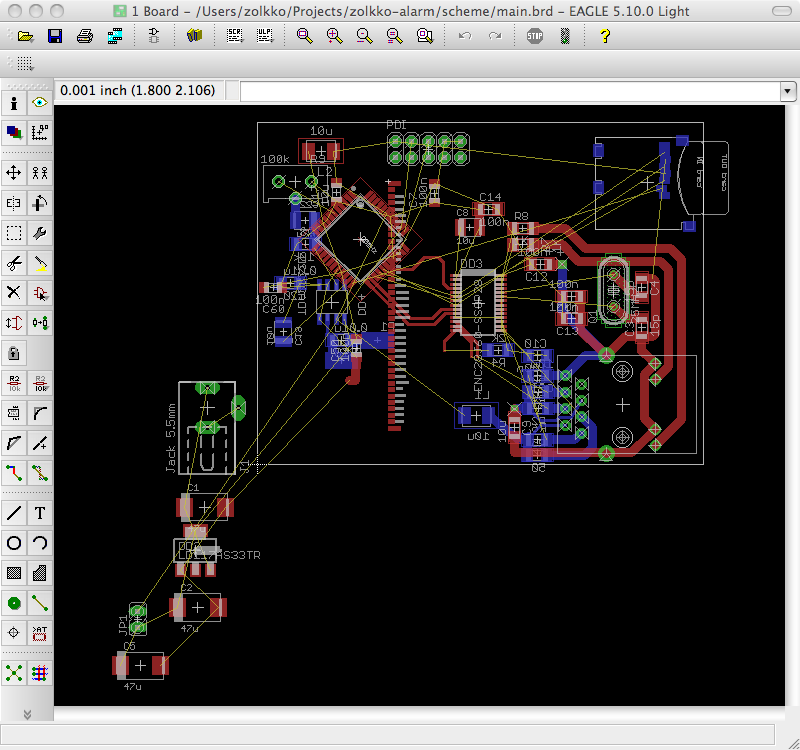
\includegraphics[bb=0 0 800 800, clip, scale=0.3]{eagle_brd.png}}
            \caption{Окно редактора печатных плат Eagle}
            \label{img:eagle_brd}
        \end{figure}

	
	\item{}Schematic Editor - программа для создания принципиальных электрических схем (рис. \ref{img:eagle_sch}).
		\begin{itemize}
			\item{}до 999 листов на одну схему;
			\item{}проверка эллектичских правил;
			\item{}обмен вентелей и пинов;
			\item{}возможность создания печатной платы из схемы одной командой.
		\end{itemize}
        \begin{figure}[h]
            \center{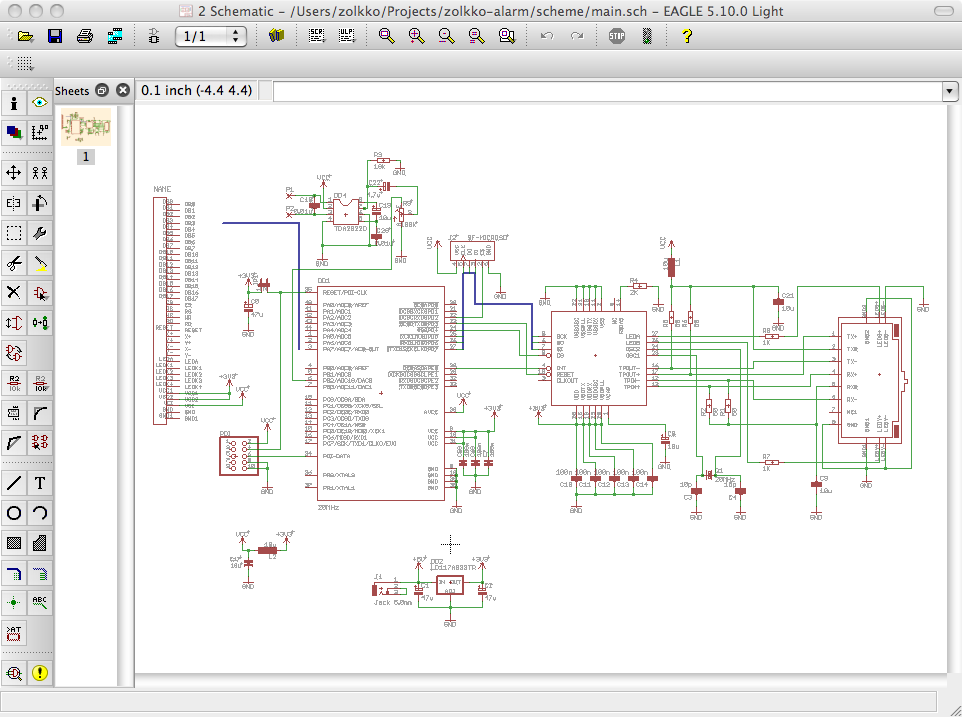
\includegraphics[bb=0 0 1010 730, clip, scale=0.3]{eagle_sch.png}}
            \caption{Окно редактора пренципиальных схем Eagle}
            \label{img:eagle_sch}
        \end{figure}
	\item{}Autorouter - программа автоматической трассировки.
		\begin{itemize}
			\item{}ripup-and-retry трассировщик - на первом проходе выполняется соединение абсолютно всех проводников без обращения внимания на возможные конфликты, заключающиеся в пересечении проводников на одном слое и нарушении зазоров. На каждом последующем проходе автотрассировщик пытается уменьшить количество конфликтов, разрывая и вновь прокладывая связи;
			\item{}до шестнадцати сигнальных слоёв;
			\item{}стратегия трассировки может быть подстроена заданием весовых коэфициентов.
		\end{itemize}
\end{enumerate}

Все эти программы встроены в один пользовательский интерфейс, таким образом нет необходимости в
предварительном конвертировании нет-листов.
\end{par}


\subsection{Обзор современных систем программирования микроконтроллеров}

Ведущими разработчиками 8/16 битных микроконтролеров на сегодняшний день
являются компании:
\begin{itemize}	
	\item{} Microchip Technology Inc. -- выпускающие микроконтроллеры семейства PIC и
		сигнальные микроконтроллеры dsPIC,
		получивших широкое распространение в странах серевной и южной америки.
		Отличительной особенностью PIC--контроллеров является хорошая преемственность
		различных семейств.
		8-битные микроконтроллеры представлены двумя базовыми архитектурами ядра:
		BASELINE и MID-RANGE. Основным инструментом разработки является среда программирования
		MPLab и набор компиляторов GCC.
	\item{} STMicroelectronics -- европейская компания, активно продвигающая свои 8 и 32
		разрядные микроконтроллеры на рынке. В качестве среды разработки предлагается
		использовать адаптированную версию набора компиляторов GCC.
	\item{} Texas Instruments --специализирующаяся на выпуске цифровых сигнальных процессоров
		и наиболее удачной линейки микроконтрллеров общего назначения MSP430.
	\item{} NXP Semiconductors -- производит 8 разрядные микроконтроллеры
			80C51: LPC900 и LPC700.
			Основным инструментом разработчика является адаптированная версия
			Keil PK51 Professional Developers Kit, предоставляющей инструменты для
			генерации программ для LPC, и включающая в себя среду разработки
			$\mu{}$Vision IDE, C51 ANSI C компилятор и A51 макро ассемблер, $\mu{}$Vision отладчик
			со встроенным симулятором ЦПУ и переферийных устройств. В комплект поставки
			среды так же входит внутрисхемный отладчик ISD51.			
	\item{} Freescale Semiconductor -- HC80, HC05, HC11.
	Эти микроконтроллеры используют расширенную архитектуру ЦПУ M68HC08.
	Основным иструментом разработки является CodeWarrior Development Studio, в поставку
	которой так же включается симулятор чипа и мастер автоматического генерирования
	кода ''Processor Expert''.
	\item{} Atmel Corporation -- выпускает микроконтроллеры AVR, основанные на ядре
	собственной разработки. Основное средство разработки -- AVR Studio. В начале 2011
	года компания прекратила поддержку старых версий AVR Studio 4 и AVR Studio 32,
	заместив их AVR Studio 5 -- средой разработки основанной на Microsoft Visual
	Studio Shell. В качестве компилатора выступает адаптированная версия GCC. Так
	же в комплекте среды разработки поставляется симулятор ЦПУ и переферии, и
	набор программного обеспечения ''AF''.
\end{itemize}

Таким образом, все лидирующие производители микроконтроллеров предоставляют
бесплатные системы программирования своих мкроконтроллеров.
Причём, можно отметить, что системы программирования либо основанны на коде 
набора компиляторов GNU GCC, либо в качестве стандартной среды разработки лицензируется
программное обеспечение других компаний. Во втором случае, зачастую, бесплатные
стандартные системы программирования обладают рядом ограничений, позволяющим только
опробовать демонстрационные проекты.

Однако, на рынке пристствует довольно большео число компаний специализирующихся
исключительно на создании систем программирования для встраиваемых систем. Лидером
в этой области является IAR Systems -- компания предоставляющая широчайший перечень компиляторов и стандартных библиотек для большого числа микроконтроллеров разных архитектур.
Их продукт IAR Embedded Workbench поддерживает следующие семейства микроконтроллеров:
\begin{itemize}
	\item{} 8051;
	\item{} ARM;
	\item{} Atmel AVR, AVR32;
	\item{} Freescale ColdFire, Freescale S08, Freescale HCS12;
	\item{} Maxim MAXQ;
	\item{} Microchip dsPIC/PIC24, PIC18;
	\item{} National CR16C;
	\item{} Renesas RL78, 78K, V850, H8, M16C, R8C, M32C, RX, R32C, SuperH;
	\item{} Samsung SAM8;
	\item{} STMicroelectronics STM8;
	\item{} TI MSP430.
\end{itemize}
Ещё одним интерестным продуктом этой компании является IAR visualState -- системе
программирования, автоматически генерирующей программный код на основе графически
заданного конечного автомата. При этом возможно проводить комдинированную разработку
программного обеспечения, когда часть кода программы генерируется автоматически, а часть
разрабатывается программистом.

\begin{figure}[h]
	\center{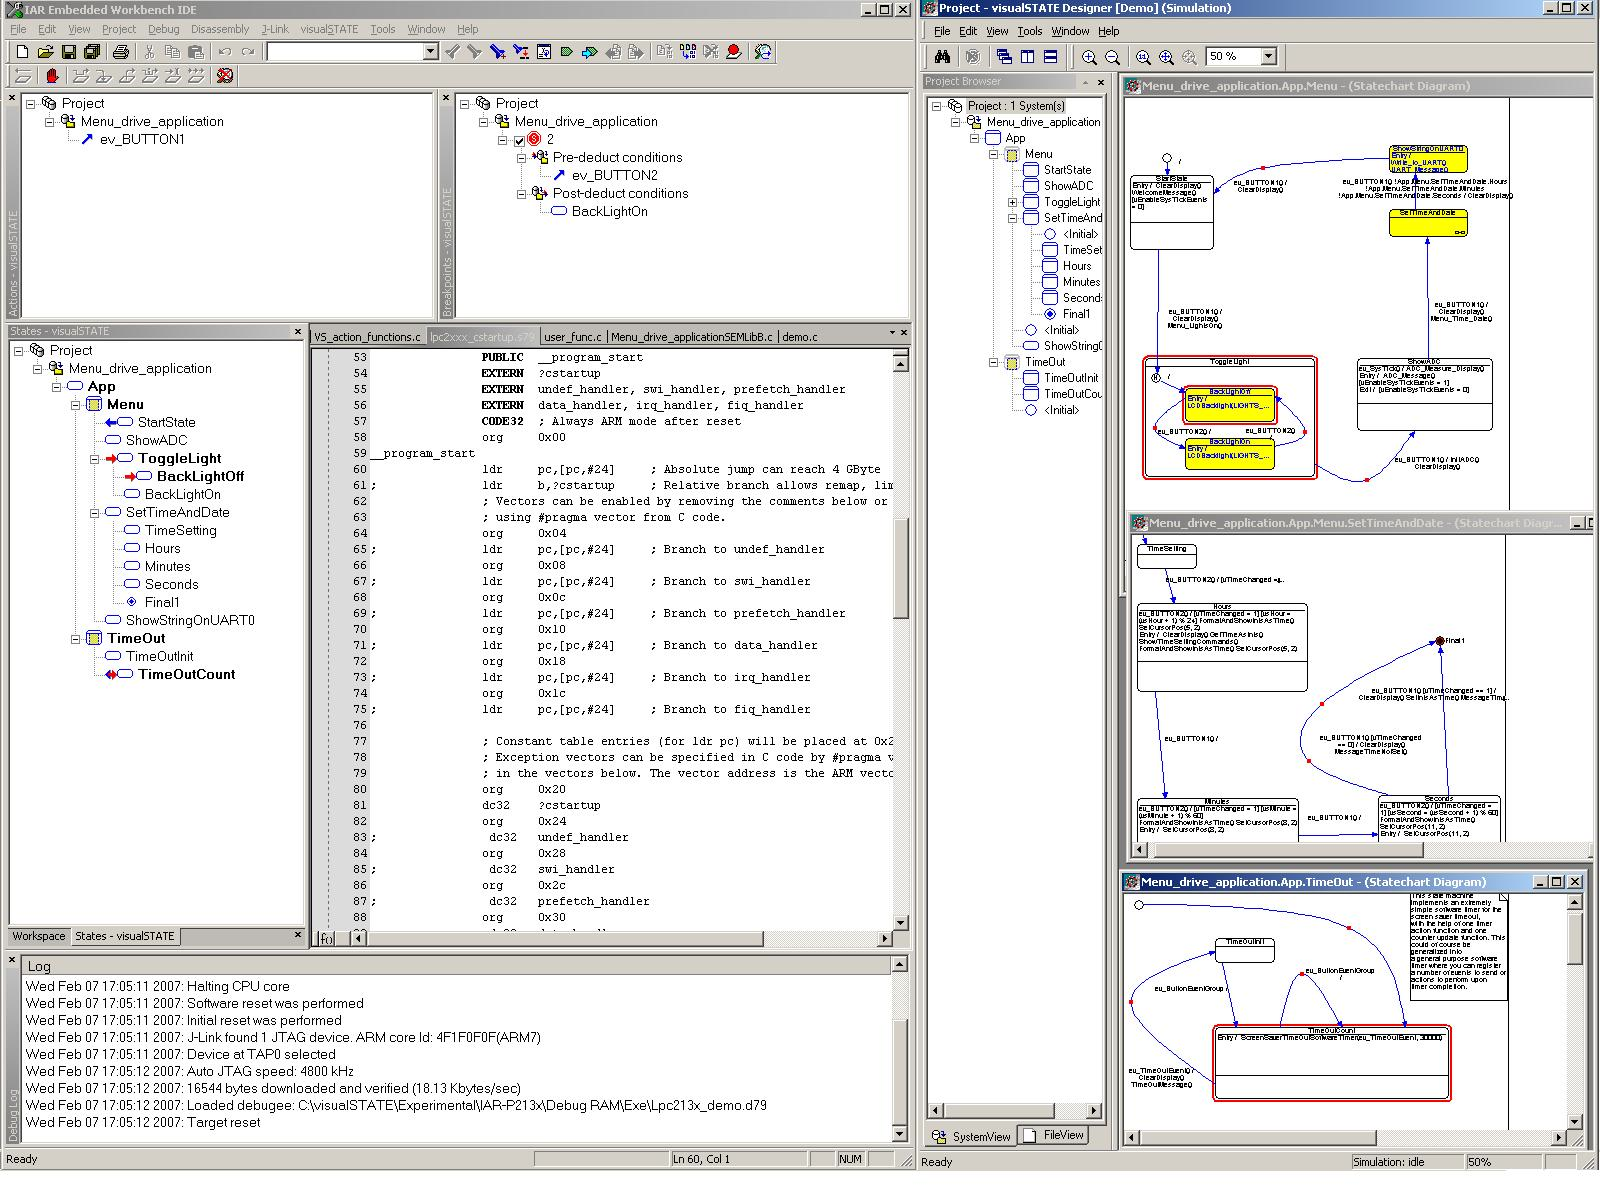
\includegraphics[bb=0 0 900 700, clip, scale=0.3]{iar_vis_state.png}}
	\caption{Среда разработки IAR visualSTATE}
	\label{img:iarVis}
\end{figure}

\newpage{}



%% Описываем выбор инструментария
%!TEX root = /Users/zolkko/Projects/zolkko-alarm/doc/main.tex
\section{Выбор инструментальных средств разработки микроконтроллерного программно-аппаратного комплекса}

\subsection{Выбор микроконтроллера}
Основными требованиями предъявляемыми мной к центральному вычислительному устройству
создаваемого устройства является:
\begin{itemize}
	\item{} невысокая стоимость;
	\item{} низкое энергопотребление;
	\item{} в число поддерживаемой переферии должен присутствовать ЦАП;
	\item{} аппаратная поддержка SPI;
	\item{} поддержка производителем этого рода устройств;
	\item{} доступность устройства;
	\item{} <<сильное>> сообщество разработчиков под эту архитектуру;
	\item{} наличие литературы и справочных материалов.
\end{itemize}


По всем этм пунктам идеально подходит микроконтрллер семейства XMega компании ATmel -- atxmega32a4.
Этот микроконтроллер полностью отвечает минимальным требованиям. В целях достижения максимальной
производительности и параллелизма у микроконтроллеров AVR используется
Гарвардская\\*
архитектура (рисунок \ref{img:avr_arch}) с отдельными памятью и шинами программ и данных. Инструкции,
хранящиеся в памяти программ, выполняются на одноуровневом конвейере. Это означает, что
во время выполнения одной инструкции выполняется предварительная выборка из памяти программ
следующей инструкции. Данная концепция делает возможным выполнение по одной инструкции за
каждый цикл синхронизации.

\begin{figure}[ht]
	\center{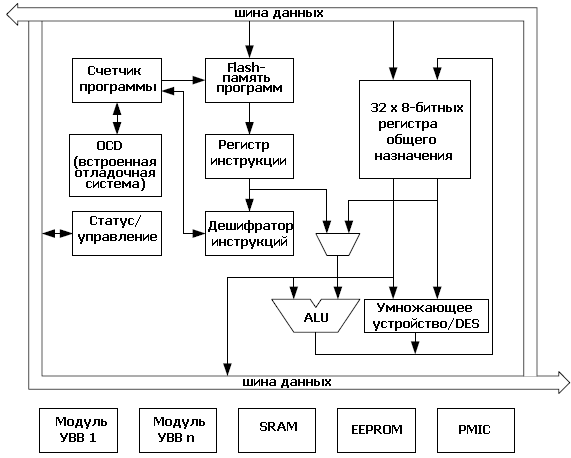
\includegraphics[bb=0 0 590 460, clip, scale=0.6]{avr_arch.png}}
	\caption{Архитектура AVR}
	\label{img:avr_arch}
\end{figure}


Так же в случае необходимости может быть заменён на более мощьный микроконтроллер того же семейства.
Для обеспечения этого функционала компания Atmel предприняла ряд шагов.

\begin{par}
    1. Была реорганизована область памяти, таким образом, чтобы все связанные между
            собой регистры располагались в памяти строго последовательно.
\end{par}
\begin{par}
    2. Была переписана стандартная библиотека C/C++, так чтобы обеспечивалась
            максимальная переносимость кода написанного для одного микроконтроллера
            на другой микроконтроллер того же семейства.
\end{par}

Микроконтроллеры серии XMega обладают следующими характеристиками:
\begin{itemize}
	\item{} 8/16-разрядное высокопроизводительное RISC ЦПУ AVR;
	\item{} 138 инструкций;
	\item{} аппаратное умножающее устройство;
	\item{} 32 8-битных регистра, напрямую подключенные к АЛУ
	\item{} прямая адресация до 16 Мбайт памяти программ и 16 Мбайт памяти данных;
	\item{} полная поддержка 16/24-битного доступа к 16/24-битным регистрам ввода-вывода;
	\item{} эффективная поддержка 8-, 16- и 32-битных арифметических инструкций;
	\item{} защита от изменения настроек критических функций системы.
\end{itemize}

Помимо этого, по сравнению с предыдущим семейством Mega \cite{avrref}, в микроконтроллеры семейства
XMega был внесен ряд значительных изменений.

\begin{par}
    1. Свехмалое энергопотребление обеспечиваемое технологией picoPower второго поколения.
    picoPower позволяет еще больше улучшить эффективность использования батарейного источника.
    То, что микроконтроллеры гарантируют нормальное функционирование при напряжении 1.6 В означает,
    что, например, в составе мобильных телефонов, они могут быть запитаны от стабилизированного
    источника напряжением 1.8В 10\%, тем самым, позволяя снизить себестоимость системы и увеличить
    длительность работы от батарейного источника. 
\end{par}

\begin{par}
    2. Event System -- позволяет организовать передачу данных между встроенными периферийными
    устройствами без вмешательства ЦПУ или использования ПДП.
    Этим гарантируется 100\% предсказуемость и малое время реагирования.
    До 8 одновременных событий или условий прерывания в периферийных устройствах могут автоматически
    инициировать действия в других периферийных устройствах \cite{avrxm}.
\end{par}

\begin{par}
    3. 12-разрядные АЦП и ЦАП. Для обеспечения высокоточной обработки аналоговых сигналов в состав 
    микроконтроллеров XMEGA интегрированы 12-битные преобразователи аналоговых сигналов. АЦП
    микроконтроллеров XMEGA могут достигать частоты преобразования до 2 МГц, что делает их самыми
	быстродействующими и точными на фоне АЦП обычных микроконтроллеров.
	Поскольку микроконтроллеры XMEGA также интегрируют два 12-битных ЦАП на частоту преобразования
	до 1 МГц и четыре усовершенствованных аналоговых компаратора, это делает их лидерами по
	степени интеграции компонентов для аналоговой обработки.
\end{par}

\begin{par}
   4. Расширена функциональность портов ввода-вывода общего назначения. Каждый из портов
    ввода-вывода может быть сконфигурирован как источник внешнего прерывания, при этом событие внешнего прерывания
    может минуюя ЦПУ запускать обработку данных используя модуль прямого доступа к памяти. \\*
    Новыми доступными состояниями портов ввода-вывода стали totem-pull, bus-keeper, wired-or, wired-and.
\end{par}


\subsection{Язык программирования микроконтроллера}
\begin{par}
Микропрограммы для микроконтроллеров XMega можно писать на нескольких языках программирования.
Сама компания Atmel предоставляет для программирования своих устройств два средства разработки:
	\begin{enumerate}
		\item{}AVR assembler -- язык низкого уровня, транслирует исходный код пользовательской
                программы в объектны и исполняемый код, его применение позволяет
                добиться от программы наибольшей производительности;
		\item{}AVR-GCC -- кодогенератор и набор дополнительных утилит для Gnu C Compiller от
                компании Atmel, активно поддерживаемый сообществом разработчиков, а так же
                входящий в комплект среды разработки AVR Studio, AVR32 Stdio и
                распростроняемый на правах свободного программного обеспечения, в состав
				которого входят компиляторы языка C и C++.
	\end{enumerate}
\end{par}

\begin{par}
В начале 2011 года компания предоставила новую версию своей интегрированной системы
разработки - AVR Studio 5. В отличии от предшественника, новая система позволяет разрабатывать
программное обеспечение для всех семейств микроконтроллеров AVR используюя единую среду разработки.
\end{par}

\begin{par}

\begin{figure}[ht]
	\center{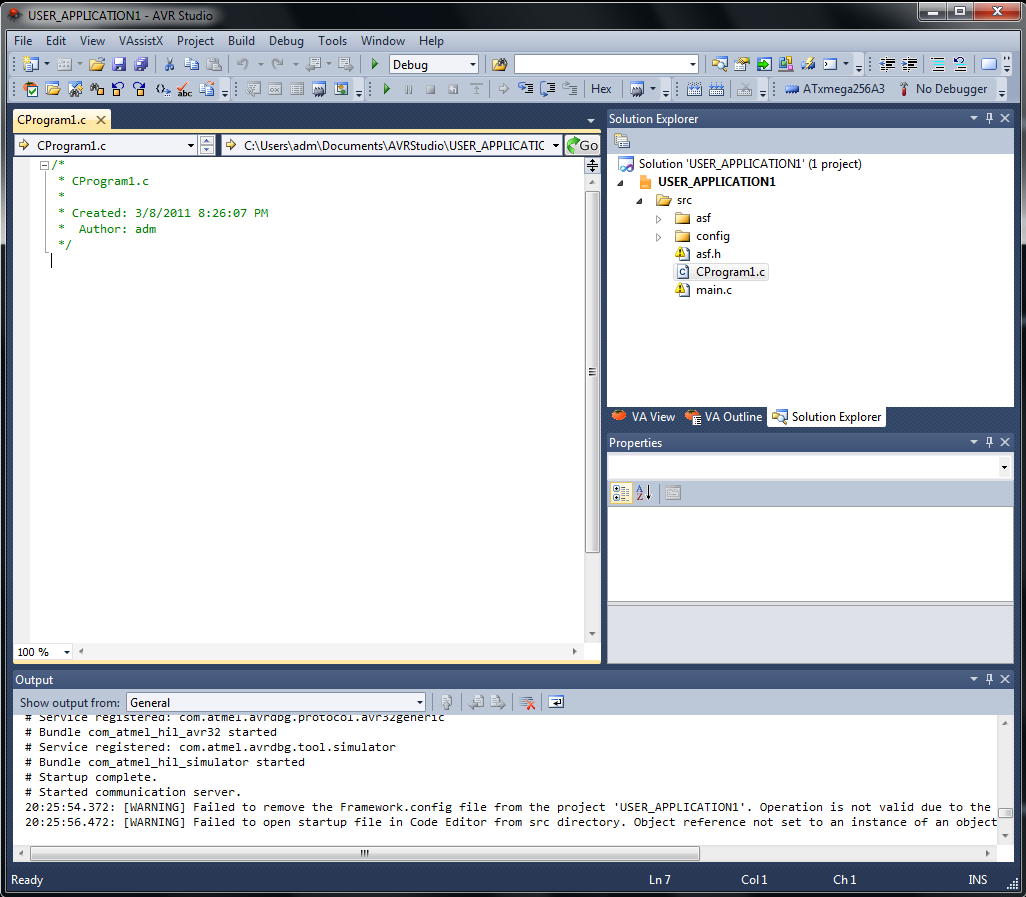
\includegraphics[bb=0 0 800 700, clip, scale=0.5]{avrstudio5.png}}
	\caption{AVR Studio 5}
	\label{img:avr_studio}
\end{figure}


Новая среда разработки AVR Studio 5 (рисунок \ref{img:avr_studio}) основана на базе лидирующего
продукта -- Microsoft Visual Studio.
И так же как и предшественники, новая версия AVR Studio 5  распространяется бесплатно.
В качестве компилятора и кодогенератора в AVR Studio 5 по прежнему используется AVR-GCC,
что позволяет продолжать использовать уже существующие наработки.
\end{par}

\begin{par}
Считается \cite{avrev}, что для разработки эффективного встраиваемого приложения для 8-битных микроконтрллеров
AVR наиболее целесообразно применять язык ассемблера или в случае, когда необходимо добиться
большей читаемости и поддерживаемости приложения -- язык С.
Однако, лидирующая группа японских производителей ЦПУ, возглавляемая NEC, Hitachi, Fujitsu и Toshiba,
разработала специализированных диалект языка C++ --- Embedded C++ (EC++), позволяющий применять
C++ для встраиваемых систем. Основная цель разработки --- перенос существующих методологий и шаблонов
программирования C++ в облать применения встраивамых систем.
При этом программы код генерируемых компиляторами EC++ может даже дать приемущества по сравлению
с языком C. Так как сама структура языка C++ позволяет минимизировать объём кода и одновременно
повышая его эффективность.
\end{par}

\begin{par}
Однако, при выборе в качестве языка программирования C++, из текущей реализации поставляемой с AVR-GCC,
необходимо учитывать некоторые её ограничения.
\end{par}

\begin{par}
 	1. В наборе компиляторов AVR-GCC отсутствует стандартная библиотека C++.
\end{par}

\begin{par}
	2. Необходимо помнить, что EC++ -- это только подмножество C++, по этому некоторые особенности языка были
        убраны из стандарта:
        \begin{itemize}
            \item{} множественное наследование;
            \item{} базовые виртульаные классы;
            \item{} информация времени исполнения;
            \item{} приведение типов (static\_cast, dynamic\_cast, reinterpret\_cast и const\_cast);
            \item{} квалификаторы типов;
            \item{} пространства имён;
            \item{} исключения;
            \item{} шаблоны.
        \end{itemize}
\end{par}



\subsection{Выбор языка программирования сетевого сервиса}

При проектировании сетевого сервиса от инструментального средства ожидается, чтобы оно
отвечало следующим требованиям \cite{technob}:

\begin{enumerate}
	\item{} инструментальное средство должно быть высокого уровня --- язык высокого уровня,
            освобождает разработчика от рутинной работы вроде ручного выделения и освобождения
            памяти, и позволяет ему сфокусироваться на оперировании абстракциями предметной области;

	\item{} язык должен минимизировать количество ошибок которые может допустить программист в
             процессе разработки системы;

	\item{} высокая степень параллелизма -- необходима возможность обслуживать тысячи клиентов
            одновременно;
	
	\item{} отказоустойчивость -- телеком-системы слишком масштабны, чтобы самому разработчику
             имело смысл даже пытаться предусмотреть все возможные ошибки;
	
	\item{} возможность обновления кода сервиса без останова выполнения программы;
	
	\item{} наличие обширной системной библиотеки,  а так же предопределённых каркасов
            проектов задающих общую структуру создаваемой системы, что позволяет ещё
            на этапе проектирования системы оценивать её будущие качества, а так же избавляет разработчика
			от необходимости реализовывать типовые решения самостоятельно, при этом тратя время на
			тестирование и отладку системы.
\end{enumerate}

\begin{par}
Один из немногих существующих и поддерживаемых на сегоднешний день языков программирования
отвечающих всем этим требованиям является Erlang и платформа Open Telecom Platform (OTP).
\end{par}

\subsubsection{Обзор языка Erlang и платформы OTP}

\begin{par}
В середине 1980-х, Ericsson Computer Science Laboratory было дано задание: исследовать языки
программирования подходящие для разработки телекоммуникационных продуктов нового поколения.
Джой Армстронг(Joe Armstrong), Роберт Вирдинг (Robert Virding) и Майк Вильямс (Mike Williams) под
руководством Брайна Декера (Bjarne Dacker) потратили два года на прототипирование
телекоммуникацинного приложения поочерёдно  используя все доступные на тот момент языки и
системы программирования. В результате, несмотря на то, что многие языки программирования обладали
интересными и подходящими свойствами, ни один из них не удовлетворял всех их требованиям. В результате
они приняли решение создать их собственный язык программирования.
\end{par}

\begin{par}
Erlang был создан под влиянием функциональных языков таких как  ML и Miranda, параллельных языков
ADA, Modula и Chill, и языка логического программирования Prolog. Erlang так же унаследовал некоторые
черты таких язков как Smalltalk, проприетарных языков Ericsson EriPascal и PLEX \cite{erlang}.
\end{par}

\begin{par}
Используя построенную на Prolog виртуальную машину Erlang (VM), лаборатория потратила  четыре года на
прототипирование телекоммуникационного приложения с применением и постоянными доработками новго языка.
Именно из-за применения метода проб и ошибок язык Erlang стал таким, каким он является сейчас. В 1999
Майк Вильямс переписал на Си виртуальную машину, и годом позже, на этом языке был выпущен первый
коммерческий продукт. 
\end{par}

\begin{par}
История создания языка Erlang важна для понимания его философии, так как в отличии от других языков,
которые находили свою нишу уже после разработки и распространения, Erlang изначально создавался
для решения конкретных задач бизнеса. Он создавался под задачи построения распределённых,
отказоустойчивых систем реального времени массового обслуживания.
\end{par}

\begin{par}
Так как такие области как системы поддержки продаж, банковские системы, системы компьютерной
телефонии, системы интеграции уровня предприятий зачастую предъявляют к своему программному
обеспечению аналогичные требования, то Erlang нашёл своё применение и в них.
\end{par}

Подтверждением применимости Erlang в этих областях могут служить факты использования этого языка в
проектах компаний:
\begin{itemize}
	\item{} Amazon -- использует Erlang для реализации SimpleDB, предоставления системы
        управления базами данных как части Amazon Elastic Compute Cloud (EC2);
	\item{} Yahoo! -- использует Erlang для реализации своего сервиса социальных закладок,
    который обслуживает более 5 милионов пользователей и 150 милионов URL;
	\item{} T-Mobile -- использует Erlang в их SMS и авторизирующей системах;
	\item{} Motorola -- использует Erlang в системе обработки звонков системы обслуживания клиентов;
	\item{} Ericsson -- использует Erlang для поддержки узлов используемых в GPRS и 3G
    мобильных сетях по всему миру;
	\item{} Facebook и Yandex -- используют написанный на Erlang сервер мгновенных
    сообщений Ejabberd.
\end{itemize}



%% Реализация автоматизированной программно-аппаратной системы управления коптильной камерой
%!TEX root = /Users/zolkko/Projects/zolkko-alarm/doc/main.tex
\section{Реализация программно-аппаратного универсальной
системы терморегулирования на базе микроконтроллера AVR семейства XMega}
В качестве объекта исследования в ходе выполнения дипломного проектирования мной
была спроектирован и частично реализован программно-аппаратный комплекс
универсального терморегулирования.

Одной из возможных областей применения такого рода комплексов является дистанционное
автоматизированное управление коптильными камерами, используемыми при изготовлении
колбасных изделий фабрик пищевой промышленности.

\subsection{Описание структурной схемы универсальной системы терморегулирования}
Структурная схема универсальной системы терморегулирования на базе микроконтроллера
AVR семейства XMega приведена в приложении A.

Функциональным назначением представленных на схеме блоков является:
\begin{enumerate}
	\item{} Управляющее устройство -- устройство устанавливаемое непосредственно
	на объект управления. Выполняет следующие функции:
		\begin{itemize}
			\item{} ОУ -- чтение показаний термопар и усиление их сигнала;
			\item{} устройство индикации -- выводит информацию о текущем состоянии системы;
			\item{} память -- хранит настройки системы и список технологических процессов для
				исполнения;
			\item{} звуковая сигнализация -- выполняет оповещение звуковым сигналом о
				наступлении события завершения текущей операции или о том, что произошла ошибка;
			\item{} устройство ввода -- обеспечивает функцию задания операции на исполнение,
				остановку операции исполнения;
			\item{} датчик температуры -- получение температур холодного спая термопары;
			\item{} блок ШИМ управления -- формирует управляющий сигнал, воздействующий на
				тепло-электро нагреватель;
			\item{} сетевой интерфейс -- обеспечивает функцию передачи и приёма данных
				через сеть Ethernet 802.3;
			\item{} центральный процессов -- модуль обеспечивающий взаимодействие компонентов
				управляющего устройства, направленное на исполнение заданного технологического
				процесса.
		\end{itemize}
	\item{} Контролирующий сервис -- обеспечивает:
	 	\begin{itemize}
			\item{} авторизацию устройства управления;
			\item{} сбор и хранение показаний датчиков управляющего устройства;
			\item{} интерфейс пользователя контролирующей системы.
		\end{itemize}
	\item{} Объект управления -- объект, управление и контроль состояния которого необходимо проводить
		в данном технологическом процессе.
\end{enumerate}


\subsection{Детализация компонентов универсальной системы терморегулирования}
Схема управляющего устройства реализуется на следующих компонентах:

\begin{enumerate}
	\item Центральный микроконтроллер -- микроконтроллер atxmega128a3. Микропрограмма контролера
	составлена таким образом, что прерывание модуля RTC происходит с частотой 100 Гц.
	При приходе прерывания микроконтроллер отсчитывает количество $ \frac{1}{100} $ с. прошедших с момента
	включения схемы и выполняет запрос на обновление состояния всех дочерних объектов.
	Программа микроконтроллера написана на языке C++ для компилятора входящего в поставку
	AVR-GCC 4.3.3.
	
	\item В качестве устройства индикации используется TFT ЖК-дисплей DST\-2001\-PH \cite{display} со встроенным
	драйвером ili9320 включённым в режиме system i80 16-бит\cite{ili9320}.
	Так как количество портов ввода\--вывода на используемом микроконтроллере достаточно, введение дополнительных узлов
	расширяющих возможности ввода\--вывода микроконтроллера -- не предусмотрено.
	\begin{figure}[ht]
		\center{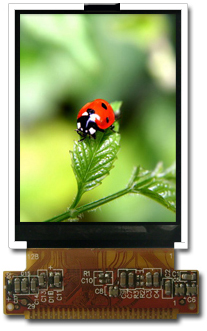
\includegraphics[bb=0 0 150 250, clip, scale=0.5]{ili9320.png}}
		\caption{Внешний вид TFT ЖК-дисплея DST2001PH}
		\label{img:iili9320}
	\end{figure}
	
	\item Модуль ввода данных пользователя выполнен на сенсорном экране ЖК-дисплея,
	выполненного по 4-проводной схеме включения резистивного сенсорного экрана. Для
	оцифровки значений получаемых с сенсорного экрана должны использоваться АЦП\cite{avradc} центрального
	микроконтроллера.
	
	\item Звуковое оповещение о наступившем событии выполнено на широко распространённой
	микросхеме mc34119, включённой в стандартном режиме (рис. \ref{img:mc34119m}).
	\begin{figure}[ht]
		\center{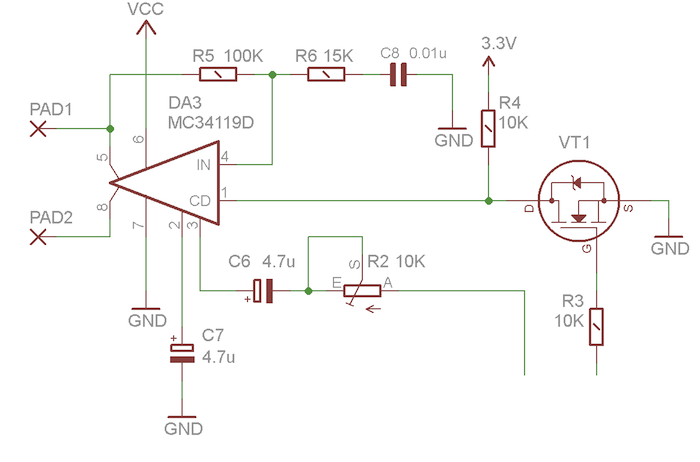
\includegraphics[bb=0 0 700 480, clip, scale=0.5]{mc34119.png}}
		\caption{Схема включения mc34119}
		\label{img:mc34119m}
	\end{figure}
	Управление сигналом Chip Disable микросхемы производиться ключом на транзисторе VT1. Низкий уровень
	переводит микросхему в состояние низкого энергопотребления \cite{mc34119}.
	
	Для надёжного перехода микросхемы усилителя необходимо производить выдержку не менее 40 мс.
	Сигнал на УНЧ подаётся с цифро-аналогового преобразователя микроконтроллера.
	
	\item В качестве памяти устройства используется энергонезависимые карты памяти MicroSD.
	Применение этого вида памяти позволяет не прибегая к перепрограммированию устройства
	вносить конфигурационные данные в систему. В случае недоступности внешней памяти микроконтроллер использует
	встроенную память EEPROM.
	
	\item В качестве контролера сетевого интерфейса используется микросхема фирмы Micro Chip
	enc28j60. Пример включения этого микроконтроллера дан на рисунке \ref{img:ienc28j60}.
	\begin{figure}[ht]
		\center{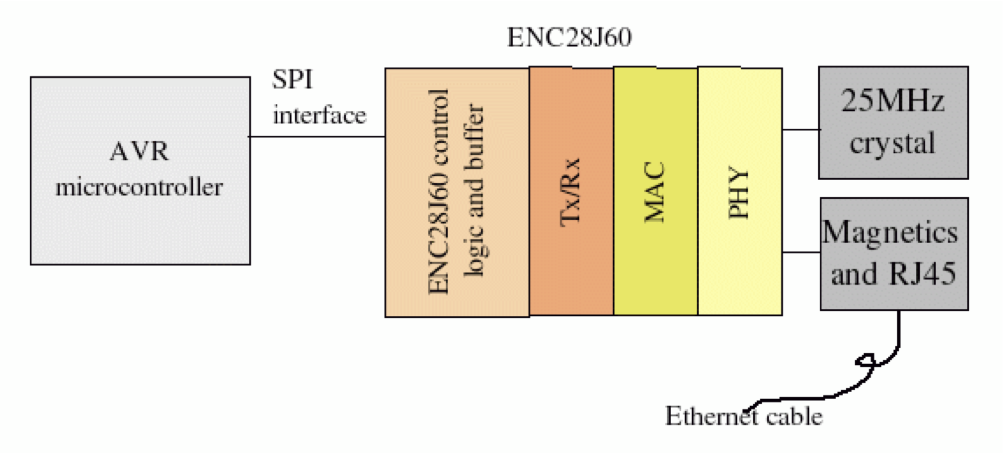
\includegraphics[bb=0 0 500 220, clip, scale=0.6]{enc28j60.png}}
		\caption{Схема включения микроконтроллера enc28j60}
		\label{img:ienc28j60}
	\end{figure}
	
	Этот микроконтроллер требует использования трансформатора с отношением 1:1 сертифицированного
	для сетей 10base-T. По этому для упрощения изделия необходимо использовать готовые RJ45
	коннекторы ''Magjack'', которые включают в своей конструкции необходимые трансформаторы и
	свето диоды. В случае использования этого метода в схему устройства необходимо будет добавить
	только одну индуктивность в 10 мкГн.
	
	Взаимодействие центрального микроконтроллера и микросхемы сетевого интерфейса осуществляется
	по протоколу SPI \cite{enc28j60}, расширенному дополнительными сигнальными линиями. Методика
	использования модуля SPI приведена в официальной документации \cite{avrspi}.
\end{enumerate}


\subsection{Анализ динамики работы системы}
В процессе разработки любой системы крайне важным шагом является проведение анализа динамики
работы разрабатываемой системы.
В качестве инструмента анализа динамики программных систем часто используются диаграммы последовательности (рис. \ref{img:dynamic}),
так как они являются удобным средством для обозначения очерёдности следования сообщений от одного объекта к другому во времени.
\begin{figure}[ht]
	\center{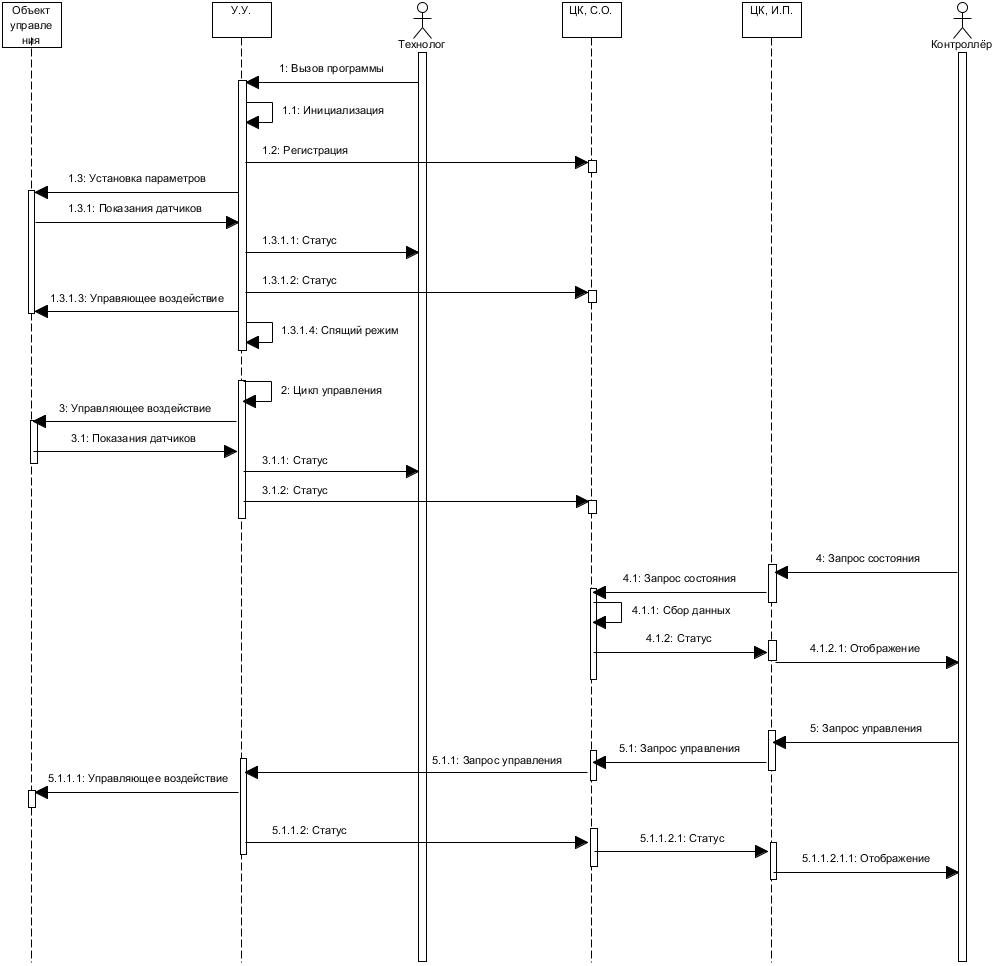
\includegraphics[bb=0 0 250 250, clip, scale=1.8]{system_dynamic.png}}
	\caption{Диаграмма динамики системы}
	\label{img:dynamic}
\end{figure}
Главный акцент диаграммы последовательности -- порядок и динамика поведения, то есть как и в каком порядке происходят события.

\subsection{Разработка контролирующего сервиса}
Из представленной диаграммы динамики работы системы (рис. \ref{img:dynamic}), видно,
что контролирующий сервис выполняет обработку исключительно коротких запросов. Однако, количество таких
запросов довольно большое.

Применение сервисов выделяющих на обработку каждого запроса отдельного потока может привести к
ситуации, когда политика операционной системы заблокирует выделение дополнительного потока сервису,
или постоянное переключение между выполняющимися равнозначными потоками приводит к значительным задержкам
в обработке одного запроса, из-за больших накладных расходов на переключение контекстов операционной системы.

В случае использования сервисов с выделенным ограниченным пулом потоков возможно возникновение ситуации, когда
из-за большого наплыва запросов, используемый пул потоков исчерпывается и сервис вынужден ставить вновь
пришедший запрос в очередь, что так же сказывается на скорости реакции системы.

Одним из возможных способов решения обозначенных проблем является применение <<лёгких>> потоков и написание кода
обработчиков сетевых запросов таким образом, что бы не возникала необходимость производить их синхронизацию.


Наиболее простым и эффективным способом добиться этого -- является применение специализированных библиотек или
систем программирования. Язык программирования ErLang изначально проектировался для решения проблем
многопоточности. А разработанная в его рамках и технология OTP, не только обеспечивает хорошую структурируемость
системы, но и позволяет производить горизонтальное масштабирование всей системы за счёт распределения нагрузки
между несколькими узлами.

Структура разработанного контролирующего сервиса представлена на рисунке \ref{img:otpStruct}.
\begin{figure}[ht]
	\center{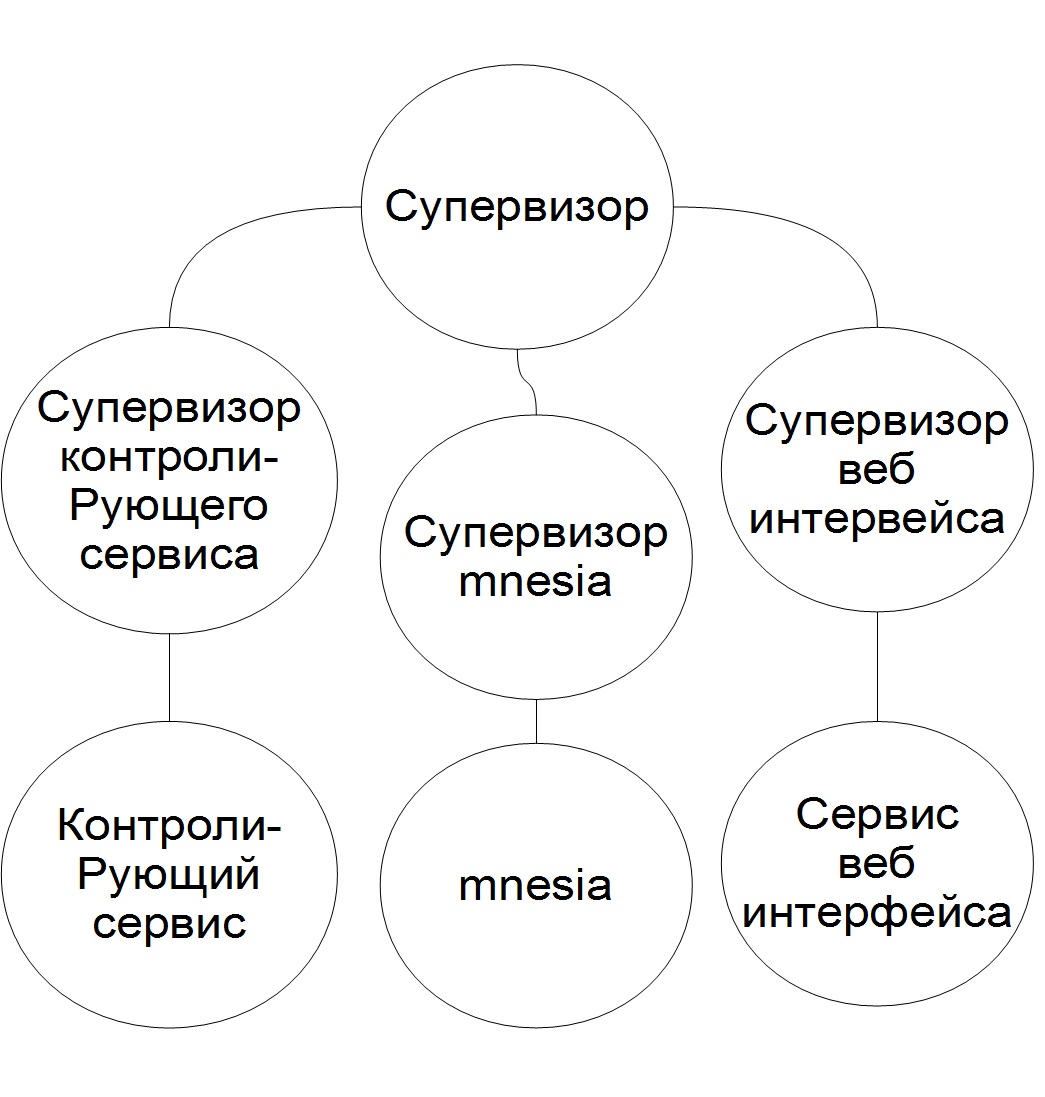
\includegraphics[bb=0 0 850 800, clip, scale=0.4]{otp_struct.png}}
	\caption{Дерево контроля контролирующего сервиса}
	\label{img:otpStruct}
\end{figure}

Система состоит из трёх рабочих процессов:
\begin{enumerate}
	\item конролирующий сервис -- обеспечивающий взаимодействие с устройствами управления;
	\item сервис базы данных -- приложение распределённой докумен-ориентированной базы данных,
	хранящей журнал выполненных операций, список опрашиваемых узлов и прочие параметры,
	необходимые для функционирования системы;
	\item веб-сервис -- серверное приложение предоставляющее интерфейс пользователя (оператора).
	к функциям.
\end{enumerate}

Каждый из рабочих процессов контролируется своим собственным супервизором, каждый из которых управляется
корневым супервизором.


\subsubsection{Методика обеспечения отказоустойчивости контролирующего сервиса}
Основной концепцией в Erlang/OTP является дерево контроля. Это модель структурирования процессов,
основанная на идее рабочих и контролеров \cite{otpOv}.

\begin{itemize}
	\item рабочие -- это процессы, которые выполняют вычисления, и, собственно, выполняют основную работу;
	\item супервизоры -- это процессы, которые контролируют поведение рабочих;
	\item дерево контроля -- это иерархическое разделение кода на контролеров и рабочих,
		позволяющее разрабатывать устойчивое к ошибкам программное обеспечение.
\end{itemize}

В случае возникновения ошибки в программном обеспечении написанном в соответствии с приведённой структурой,
супервизор произведёт перезапуск рабочего процесса. Политика реакции на ошибки определяется во время регистрации
рабочих процессов в супервизоре при его создании.

Ещё одним плюсом использования такой архитектуры сервисов является возможность распределения
сетевых служб по зонам безопасности. То есть контролирующий сервис и приложение базы данных можно разворачивать
в безопасной сетевой зоне, доступ в которую есть только у внутренних ресурсов. Веб-сервис же можно разворачивать
в демилитаризованной зоне, не опасаясь, что злоумышленник причинит вред приложению.

Не маловажным является и возможность осуществления двойного контроля выполняемых действий. На первом шаге
веб-сервис выполняет проверку правильности ввода пользователя, на втором -- контролирующий сервис
может произвести проверку адекватности выполняемых функций.


\subsection{Разработка сервиса обслуживания запросов операторов системы}
В целях обеспечения надёжности функционирования контролирующего сервиса, что обеспечивается его
 изоляцией в локальной сети предприятия, функции предоставления интерфейса пользователя оператора
и обслуживания запросов операторов были реализованы в дополнительном веб-сервисе.

В отличии от контролирующего сервиса, необходимости ограничивать доступ к веб-сервису из внешних
сетей отсутствует, так как он не позволяет осуществлять ни каких деструктивных функций
операторам системы. Его взаимодействие с базой данных состояния системы осуществляется только по чтению,
а все запросы на управляющие устройства проводятся исключительно через контролирующий сервис.

Как и контролирующий сервис, веб-сервис написан на языке программирования ErLang с использованием технологий
OTP. Подход при котором в качестве веб-сервиса используется частная реализация службы, а не готовый веб-сервис
общего назначения, позволяет повысить производительность системы, уменьшить время её отклика, за счёт реализации
только минимально необходимой для функционирования логики.

Применение архитектуры OTP при разработке веб-сервиса так же позволяет в случае необходимости горизонтальной
распределить нагрузку.

Горизонтальное масштабирование веб-сервиса можно произвести следующими способами:
\begin{itemize}
	\item создание нескольких веб-сервисов на разных сетевых интерфейсах работающих с одним экземпляром
		контролирующего сервиса;
	\item создание одного веб-сервиса, но нескольких узлов с логикой обратного вызова веб-сервиса;
	\item создание нескольких узлов веб-сервисов, каждый из которых обслуживает свой собственный узел
		контролирующего сервиса.
\end{itemize}


Веб интерфейс оператора (рис. \ref{img:acsIf}) контролирующего сервиса позволяет использовать в качестве
ПЭВМ контролирующего сервиса практически любой современный компьютер, в том числе планшетные компьютеры, нет-топы.
За счёт этого, возможно сократить количество дополнительного оборудования, необходимого для обслуживания и использования
системы при её внедрении.

\begin{figure}[ht]
	\center{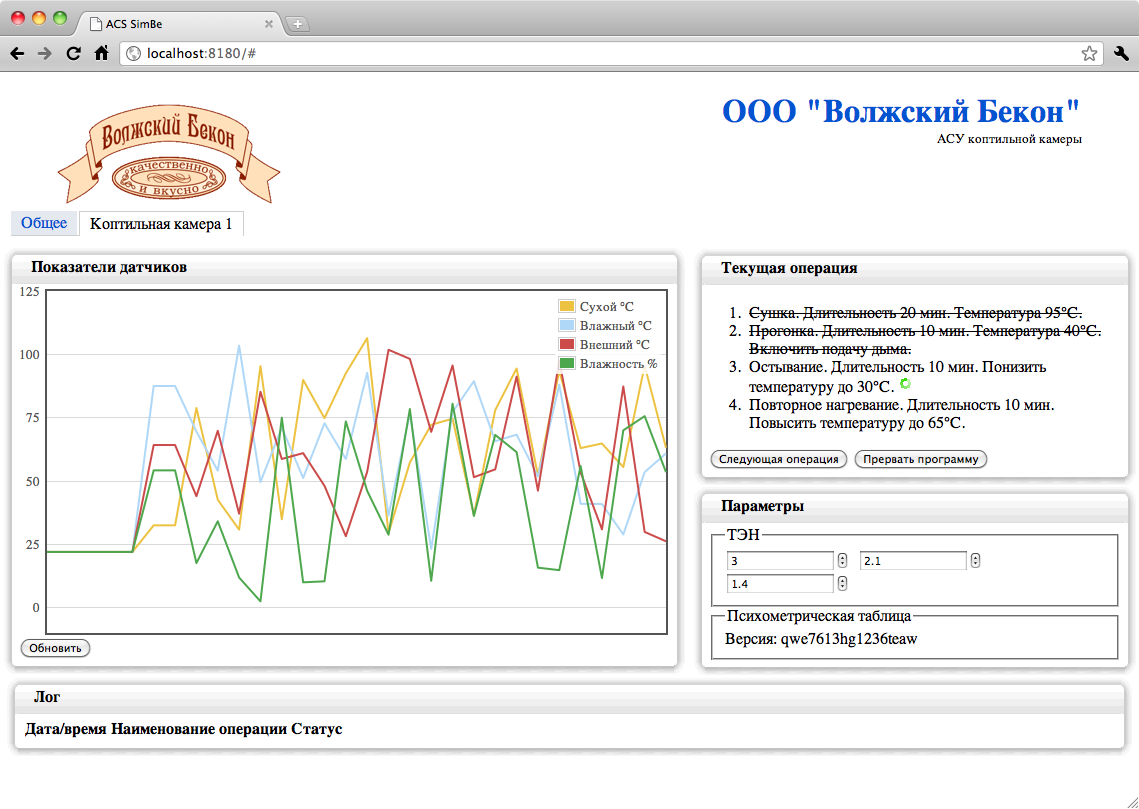
\includegraphics[bb=0 0 1200 800, clip, scale=0.4]{acs_if.png}}
	\caption{Интерфейс оператора контролирующего сервиса}
	\label{img:acsIf}
\end{figure}

\subsubsection{Виды доступных операций}
Интерфейс оператора контролирующего сервиса предоставляет следующие функции:
\begin{itemize}
	\item получение списка опрашиваемых коптильных камер;
	\item добавление коптильной камеры в список опроса;
	\item удаление коптильной камеры из списка опроса;
	\item просмотр динамики показателей датчиков;
	\item установка параметров датчиков;
	\item просмотр версии температурной таблицы;
	\item просмотр версии психометрической таблицы;
	\item просмотр списка подзадачь текущей операции;
	\item переход к следующей подзадаче;
	\item остановка выполнения операции;
	\item просмотр журнала выполненных операций.
\end{itemize}

\subsubsection{Методика оптимизации программы обслуживания операторов системы}
При разработке веб-сервиса были использованы следующие методы оптимизации:
\begin{itemize}
	\item веб-сервис на запрос пользователя выдаёт статическую html страницу, таким образом
		в отличии от типового подхода к формированию динамических веб-ориентированных приложений,
		логика веб-сервиса не выполняет динамического формирования страниц по шаблону, а следовательно
		скорость выдачи страницы пользователю ограничена только скорость выполнения дисковых операций чтения;
	\item логика веб-приложения сосредоточена в JavaScript коде статической страницы;
	\item необходимые данные и веб-сервис передаёт приложению в формате JSON,
	что обеспечивает быстрое преобразование типов данных веб-сервиса и веб-приложения;
	\item в качестве базовой JavaScript библиотеки был выбрана библиотека jQuery 1.4, однако её часть, -- JQuery UI
	для построения элементов пользовательского интерфейса не используется, а все необходимые функции реализуется
	в приложении, что позволило сократить объём передаваемых по сети данных.
\end{itemize}


\subsection{Разработка микропрограммы управляющего устройства}



\subsubsection{Описание структуры классов микропрограммы управляющего устройства}


\subsubsection{Способ расчёта показателей датчиков температур по ГОСТ Р 208.585-2001}
% (http://www.complexdoc.ru/lib/ГОСТ%20Р%208.585-2001)
В качестве температурных датчиков устанавливаемых внутри объекта управления используются
термопары. Принцип получения показания температуры термопар основан на
термоэлектрическом эффекте Зеебека. Когда концы проводника находятся при разных температурах,
между ними возникает разность потенциалов, пропорциональная разности температур.
Коэффициент пропорциональности называют коэффициентом термоэдс.

Способ получения показаний температуры устройством управления универсальной
системы терморегулирования осован на табличном методе поиска значения.
Основной его недостаток -- необходимость выделения 300 байт памяти микроконтроллера под
таблицу соответствия температуры и текущего показания термоэдс.
Однако он обладает следующими преимуществами:
\begin{itemize}
	\item{} сложность алгоритма вычисления значения температуры линейна и максимально занимает
		900 тактов;
	\item{} таблица соответствия может одновременно кодировать значение термоэдс с поправкой на
		ошибку считанного значения термоэдс, что необходимо выполнять ввиду нелинейной зависимости
		температуры и термоэдс, разброса чувствительности термопар составляющей 10-15\%, ошибки
		вносимой операционным усилителем, ошибки вносимой способом монтажа термопары на печатной плате;
	\item{} отсутствует необходимость использовать прецизионные сопротивления делителя
		напряжения операционного усилителя.
\end{itemize}

Для получения текущего значения температуры используется следующая формула:
\begin{equation}
	T_i = min_{tbl}(Adc(E_i \times{} K_{amp}) > x) 
\end{equation}
\begin{ESKDexplanation}
	\item[где ]{} $K_{amp}$ -- коэффициент усиления операционного усилителя,
	\item{} $E_i$ -- значение термоэдс,
	\item{} $T_i$ -- значение температуры,
	\item{} $Adc()$ -- функция преобразования аналогова сигнала в цифровой.
\end{ESKDexplanation}


Например для термопары типа Т, текущей температуры $1^oC$, $K_{amp}$ равным 100 и опорным напряжением
АЦП микроконтроллера 3.3 В получим:
$E_i = 0.000043$ В. Разрешение АЦП $= \frac{3.3}{2^{12}} = 0.000805$ В. Один градус температуры
кодируется $\frac{E_i \times{} K_{amp}}{\frac{3.3}{2^{12}}} = 5.34 $ значениями
беззнакового пребразования АЦП, а измеряемый диапазон температур составит от $0^oC$ до $862^oC$,
что в 4 раза превышает необходимую разрешающую способность.

\subsubsection{Методика расчёта компенсации холодного спая}
В местах подключения проводников термопары к управляющему устройству возникают дополнительные термоэдс.
В результате их действия на вход измерительной системы фактически поступает сумма сигналов от рабочей
термопары и от <<термопар>>, возникших в местах подключения.

Существуют различные способы избежать этого эффекта. Самым очевидным из них является поддержание
температуры холодного спая постоянной.

В управляющем устройстве используется техника <<компенсации холодного спая>>: температура холодного спая
измеряется датчиком температуры DS18B20, а затем величина термоэдс холодного спая программно
вычитается из сигнала термопары.

Места подключения термопары в управляющем устройстве расположены в непосредственной близости и имеют одинаковую
температуру, то есть находиться в изотермальной зоне. Датчик DS18B20 находиться в этой же зоне. Таким образом,
для компенсации холодного спая перед код чтения температуры с термопар производит чтение паказаний датчика DS18B20,
производит обратное табличное преобразование температуры в величину термоэдс градуированную по параметрам
аналого-цифрового преобразователя и выполняет вычитание этих значений.

\subsubsection{Алгоритм управления силовой нагрузкой}
Из-за того, что процесс управления тепловыми инерционными объектами характеризуется инерционным ростом
регулируемой температуры после отключения управляющего воздействия, при управлении тепловым
технологическим оборудованием возникают длительные переходные процессы и
большие амплитуды перерегулирования, в том числе с применением ПИД законов регулирования\cite{pwmbook}.

Для сокращения длительности переходных процессов и обеспечение устойчивости процесса регулирования,
в управляющем устройстве применяется адаптивный алгоритм терморегулирования предложенный в
статье ''Разработка алгоритм регулятора температуры с применением импульсного энергетического метода''
Шельпякова А.Н. и Давыдова И.А.

Применение именно этого алгоритма обусловлено:
\begin{itemize}
	\item адаптацией регулятора к объекту управления -- позволяет применять управляющее устройство
		на разнообразных;
	\item достижение регулируемой величиной уставки за минимально возможное время;
	\item удовлетворительное качество регулирования в процессе поддержания величины вблизи уставки.
\end{itemize}

Блок схема алгоритма приведена в приложении Д.


\subsubsection{Алгоритм сетевого взаимодействия управляющего устройства
с контролирующим сервером}
Для взаимодействия с контролирующим сервисом устройство управления использует сеть
стандарта Ethernet 802.3. Так как ни сам микроконтроллер at\-x\-mega\-128\-a3, ни микросхема
ecn28j60 не имеют большого буфера хранения входящих и исходящих сетевых пакетов,
было принято решение реализовать сетевое взаимодействие устройства с внешними устройствами
по упрощенной схеме итеративной обработки одного входного и одного выходного сетевого
пакета. Алгоритм сетевого взаимодействия управляющего устройства с контролирующим сервисом представлен
на рисунке \ref{img:devProto}. Из представленного алгоритма видно, что все минимально необходимые
действия для осуществления работы по сети Ethernet 802.3, сосредоточены в одном конечном автомате.

\begin{figure}[ht]
	\center{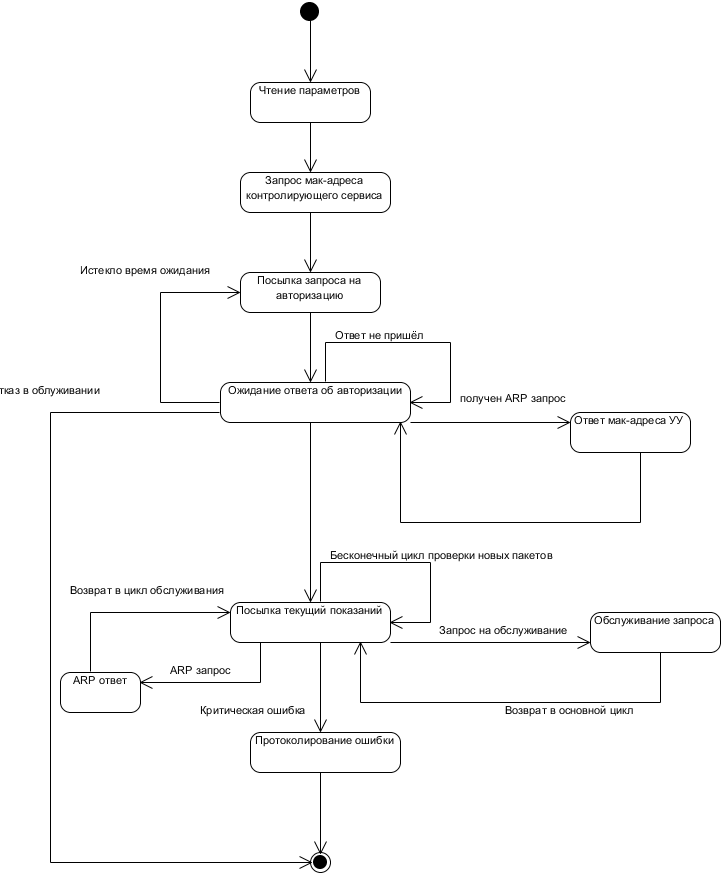
\includegraphics[bb=0 0 45 55, clip, scale=7.0]{dev_proto.png}}
	\caption{Протокол взаимодействия управляющего устройства и контролирующего сервиса}
	\label{img:devProto}
\end{figure}

Представленный конечный автомат реализует ARP ''How has'' запрос, ARP ''How has'' ответ --
минимально необходимое подмножество функций протокола ARP для работы в сетях Ethernet 802.3.
В качестве транспортного протокола передачи данных было принято решение использовать
протокол UDP, всвязи с ограниченным количеством оперативной памяти устройства управления, а так же
потому что алгоритм сетевого взаимодействия  предусматривает механизма повторения передачи
потерянных пакетов.


\subsubsection{Методика применения AES шифрования данных передаваемых
контролирующему сервису}
Одна из проблем решаемых в процессе разработки сетевого протокола 
взаимодействия управляющего устройства и контролирующего сервиса
была проблема обеспечения безопасности передаваемых данных.


Контролирующий сервис определяет, что принятые данные действительны
сравнивая пароль указанный в заголовке сетевого пакета. Однако,
при использования такого подхода, злоумышленник может прослушав
проходящий сетевой трафик получит этот пароль и использовать его
для формирования ложных запросов.


Для того, что бы избежать этого, заголовок пакета, содержащий пароль
и набор аппаратно-специфичных данных, должен подвергаться дополнительному
кодированию с использованием секретного ключа, известного только
авторизованному устройству и контролирующему сервису.


В качестве алгоритма кодирования данных заголовка пакета был использован
Advanced Encryption Standard. AES -- симметричный алгоритм блочного
шифрования, принятый в качестве стандарта шифрования правительством США
по результатам конкурса, организованного NIST в 1997 году, для замещения
алгоритма DES.


Причиной выбора именно этого алгоритма кодирования является
наличие аппаратной поддержки AES в микроконтроллерах XMega.


Благодаря наличию этого аппаратного модуля, процедура кодирования
по алгоритму AES со стороны программного обеспечения микроконтроллера
сводиться к следующим шагам:
\begin{enumerate}
    \item{} Загрузить данные ключа в область памяти $AES.KEY$
        переферийного устройства AES кодирования.
    \item{} Загрузить шифруемые данные в область памяти $AES.STATE$.
    \item{} Установить параметры шифрования и флаг $AES_START_bm$ начала
        процедуры шифрования в конфигурационном регистре $AES.CTRL$.
    \item{} Дождаться завершения шифрования, о чём сигнализирует
        флаги состояния в регистре состояния $AES.STATUS$.
    \item{} В зависимости от значения статуса, либо считать зашифрованные
        данные из области памяти $AES.STATE$, либо сообщить об ошибке
        шифрования.
\end{enumerate}


%% Адаптивный алгоритм управления температурой
\subsection{Разработка микропрограммы управляющего устройства}
Микропрограмма управляющего устройства должна выполнять следующие функции:
\begin{itemize}
    \item{} Вывод текущих показаний датчиков
    \item{} адаптивный алгоритм регулирования
    \item{} TODO:
\end{itemize}

TODO: class diagram, short description

\subsubsection{Методика понижения потребления тока устройством управления}
TODO: describe picoPower technology. \\
TODO: describe sleep walk ADC / DAC solution.

\subsubsection{Разработка адаптивного алгоритма регулятора температуры}
В качестве нагревательного элменета коптильных камер используются тепловые тенты,
включаемые в эллектрические сети общего назначения. При одна из главных проблем
которую необходимо решить при управлении таким нагревательным прибором связана
с инерционым характером роста температуры после отключения управляющего воздействия.
Из-за чего возникает длительный переходный процесс приводящий к перерегулированию.

\subsubsection{Алгоритм управления силовыми механизмами подачи влаги и дыма в коптильную камеру}

\subsubsection{Фиксация статуса выполняемой операции на удалённом конроллирующем сервере}
TODO: point that mac layer has been implemented already
TODO: describe UDP \\

\subsubsection{Модуль взаимодействия с внешней памятью}

\subsubsection{Модуль ввода-вывода управляющего устройства}

\subsubsection{Программирование микроконтрллера}



%% Разработка сервиса
\subsection{Разработка контроллирующего сервиса}

\subsubsection{Структура контроллирующего сервиса}
In this section I'm going to describe scalability features of the ACS service.

\subsubsection{Методика повышения отказоустойчивости контроллирующего сервиса}
This section is about error protection and OTP architecture.

\subsubsection{Установка контроллирующего сервиса}
IN this section I'll describe SmokeHouse service installation procedure.

\subsection{Динамика системы управления}
TODO: describe system dynamic using illustation. The main benefit is that choosed architecture
dramatically increases system scalability.


\subsection{Разработка принципиальной электрической схемы управляющего устройства в системе Eagle}
Для создания принципиальных эдектрических схем в системе Eagle используется программа
Eagle Layout Editor.

Для того, что бы открыть новое окно Eagle Layout Editor нужно вызвать команду ''Schematic''
главного меню ''New''.




\subsubsection{Подбор интегрированных баблиотек электронных компонентов}
Сильной стороной Eagle является -- обшираня коллекция библиотек поставляемых с системой.
В случае же если какой-либо необходимый компонент отстуствует в коллекции, 

\subsubsection{Ввод принципиальной электрической схемы}
\subsubsection{Выполнение контроля электрических правил}


%% экономическая часть
\section{Организационно-экономическая часть}

\subsection{Описание разрабатываемого продукта}
\begin{par}
Разработанное устройство --- <<цифровые часы с будильником>> позволяют отображать
текущее время на большём графическом жидкокристалическом дисплее. Удобным для
потребителя методом производить ввод времени срабатывания будильника.
Устройство позволяет не пребегая к перепрограммированию внутренней памяти менять
мелодию звуковой сигнализации. А так же производить синхронизацию текущего времени
с высокоточным удалённым сервером времени.
\end{par}

\begin{par}
К достоинству системы так же можно отнести то, что она реализована в соотвествии с манифестом
разработчиков открытого аппаратного обеспечения, что может прозволит повысить качество потребительских
характеристик устройства за счёт привлечения сообщества разработчиков открытого аппаратного
обеспечения. Так устройство или его часть может быть использовано в других ещё более
совершенных бытовых устройствах разрабатываемых сторонними производителями.

\begin{figure}[h]
	\center{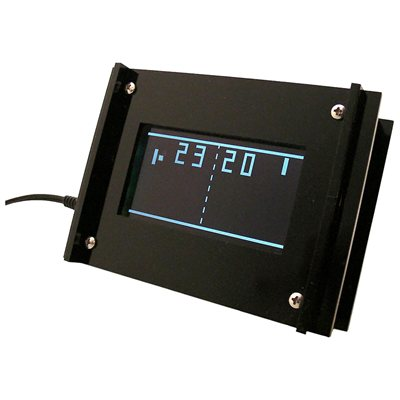
\includegraphics[bb=0 0 300 300, clip, scale=0.8]{adafruit.png}}
	\caption{Adafruit Monochron Open Source Clock kit}
	\label{img:adafruit}
\end{figure}

\end{par}

\subsection{Исследование существующих программных продуктов}
\begin{par}
Фактически на текущий момент на рынке существует только один аналог разработанного
утройства ---  Adafruit Monochron Open Source Clock kit.
Сравнительный обзор устройств представлен в таблице \ref{table:compare}.
\end{par}


\begin{par}
\begin{table}
\caption{Сравнение ''Цифровые часы с будильником'' и ''Adafruit''}
\begin{tabular}{|l|p{4cm}|p{4cm}|}
\hline{}
Характеристика & Цифровые часы с\linebreak{} будильником & Adafruit \\
\hline{}
Микроконтроллер & новое поколение AVR Xmega --- atxmega32a4 & старое семейство контроллеров AVR Mega -- atmega328 \\
\hline{}
ЖКИ & TFT 320x240 & LCD 128x64 \\
\hline{}
Метод ввода & сенсорный экран & кнопочное управление \\
\hline{}
Мелодии будильника & разнообразные мелодии выбираемые пользователем, одна встроенная мелодия & мерцание ЖКИ и звуковая сигнализация пъезоэлектрическим излучателем \\
\hline{}
Синхронизация с сервером времени & присутствует & отсутствует \\
\hline{}
Количество вариантов сборки & 1 & более 10 \\
\hline{}
Ориентировочная цена & 90\$ & 90\$ \\ 
\hline{}
Привлекательное название & отсутствует & присутствует \\ 
\hline
\end{tabular}
\label{table:compare}
\end{table}

Как видно из представленной таблицы, спректированное устройство имеет ряд преимуществт перед
устройством Adafruit. К недостаткам можно отнести только низкое число вариантов сборки устройства,
вызванное малой распространённостью разработанного устройства, что является
следствием не завершёности стадии его проектирования и разработки, а так же отстутствием каких-либо
действий нацеленных на устронение этого недостатка.
\end{par}
\newpage{}



%% бжд
%!TEX root = /Users/zolkko/Projects/zolkko-alarm/doc/main.tex
\section{Безопасность и экологичность в дипломном проекте}

\subsection{Вредные производственные факторы на рабочем месте оператора ПЭВМ}
Под рабочим местом в контексте данной работы понимается участок рабочего
помещения, оборудованный комплексом средств вычислительной техники, в
пределах которого постоянно или временно пребывает оператор ПЭВМ в прцессе трудовой деятельности.


В настоящем проекте рабочее место оператора ПЭВМ расположено в 
специально отведенном помещении .Размеры помещения : длина — 4 метра;
ширина- 3 метра ; высота потолков — 3 метра. Рабочее место включает в себя:
системный блок XTEND-11417 Intel Celeron 430;  монитор LG Flatron F700B
(электронно-лучевой);  принтер  Panasonic KX P6500 ; клавиатура A4 Terh 
G9300 Black. Кроме этого в помещении установлен оконный кондиционер
LW 05 LC.

На пользователя ПЭВМ одновременно воздействуют несколько вредных факторов.
Их источниками являются не только монитор,но и другие модули вычислительного устройства
и факторы окружающей среды. 


Основными вредными факторами являются:
\begin{enumerate}
	\item{} Электромагнитные поля и излучения.
		Дисплей по типу электронно-лучевой трубки является источником мягкого рентгеновского,
		видимого инфракрасного, ультрафиолетового, низкого и сверх
		частотного электромагнитного излучений.
	\item{} Пренапряжение зрительного анализатора.
		В обыденной жизни человек имеет дело с низкой фоновой яркостью при высокой
		контрастности предметов, и к этому в процессе эволюции приспособился наш глаз.
		При работе за дисплеем глаз считывает информацию  с излучателя, имеющего
		высокую фоновую яркость при низкой контрастности обьектов различения.
		При уменьшении яркости экрана контрастность падает, поэтому для обеспечения
		оптимального контраста необходимо повышать яркость, что увеличивает интенсивность
		вредных излучений и утомляет глаза.
	\item{} Избыточность энергетических потоков на орган зрения в оптическом диапазоне.
		Результаты исследования НИИ глазных болезней им. Гельмгольца показывают,
		что наиболее вредное влияние на пользователей в оптическом диапазоне излучений экрана
		оказывает избыточный сине-фиолетовый и синий свет этого диапазона.
	\item{} Нерациональное освещение рабочего места , повышенная блесткость и яркость на столе,
		пульсации светового потока.
	\item{} Некачественный состав воздуха рабочей зоны. Наличие пыли. Недостаток
		легких отрицательных и избыток положительных ионов.
	\item{} Гиподинамия и длительные статические нагрузки на кисти рук.
	\item{} Вибрация и шум.
	\item{} Повышенные нервные, умственные и эмоциональные нагрузки.
	\item{} Монотонность труда в сочетании с повышенным напряжением внимания и зрения.
	\item{} Опасность поражения электрическим током.
	\item{} Опасность возникновения пожара.
\end{enumerate}

\subsection{Организация рабочего места оператора ПЭВМ}
\subsubsection{Помещение}
Помещение с ПЭВМ расположено в отдельно стоящем административном здании без соприкосновения
с внешними стенами и посторонними комнатами. Трассы обычного и пожарного водоснабжения,
отопления и канализации вынесены за пределы помещения  и не находятся непосредственно над ним
на верхних этажах.


Помещение,где располагается рабочее место, оборудовано защитным заземлением в соответствии
с требованиями по технической эксплуатации. Отсутствуют линии, рядом проходящих, силовых
кабелей, создающих помехи в работе с ПЭВМ.


Площадь на одно рабочее место  составляет  12.0 кв.м. ,а обьем 31.2 кубических метра.
Звукоизоляция ограждающих конструкций отвечает гигиеническим требованиям и обеспечивает
нормируемые параметры шума (не более 50 дБА). Помещение оборудовано системой отопления и
кондиционирования воздуха . Для внутренней отделки использовались диффузноотражающие
материалы с коэффициентом отражения для потолка-0.7-0.8 ; для стен-0.5-0.6; для пола-0.3-0.5.


Для окраски стен  применялись краски холодных тонов: светло-зеленого и светло-серого цветов.
Все указанные параметры соответствуют  требованиям  санитарно-технических норм.


\subsubsection{Освещение}
В помещении с ПЭВМ  применяется комбинированное освещение: естественное и искусственное.
Естественное освещение осуществляется через светопроемы, ориентированные на  северо-восток
и обеспечивают коэффициент естественной освещенности (КЕО)не ниже 1.2 процента.
Искусственное освещение  осуществляется системой общего равномерного освещения.
Освещенность на поверхности стола в зоне размещения рабочего документа составляет 300-500лк 
Освещение не  создает бликов на поверхности экрана.


Освещенность поверхности экрана не превышает 300лк.  В качестве источников света при искусственном
освещении применяются  люминисцентные лампы с экранирующими решотками.


Общее освещение, при использовании люминисцентных светильников, 
выполнено в виде сплошной линий светильников, расположенных сбоку от рабочего места.
Рабочий стол размещен таким образом , чтобы дисплей был ориентирован боковой стороной к
световым проемам, чтобы свет падал преимущественно слева, что соответствует санитарно-техническим
нормам.



\subsubsection{Характеристика микроклимата}
Необходимым условием жизнедеятельности человека является поддержание постоянной
температуры тела благодаря терморегуляции, т. е. способности 
организма регулировать отдачу тепла в окружающую среду. Принцип нормирования
микроклимата --- создание оптимальных условий для теплообмена тела человека с окружающей
средой. Вычислительная техника является источником существенных тепловыделений, что может
привести к  повышению температуры и снижении относительной влажности.
В соответствии с требованиями СанПиН 2.2.2.542-96  (п.5.2) в помещениях с ПЭВМ  должны
соблюдаться оптимальные параметры микроклимата. Для повышения влажности воздуха следует
применять увлажнители воздуха, заправленные дистилированной водой  или свежей кипяченой
питьевой водой.


Содержание вредных химических веществ в помещении с ПЭВМ не должно превышать предельно
допустимых концентраций загрязняющих веществ в атмосферном воздухе населенных пунктов.


\subsubsection{Эргономические требования рабочему месту оператора ПЭВМ}
Проектирование рабочих мест, снабженных видеотерминалами , относится к числу важных
проблем эргономического проектирования в области вычислительной техники. Рабочее место и
взаимное расположение всех его элементов должно соответствовать антропометрическим,
физическим и психологическим требованиям. Большое значение имеет также характер работы.
В частности, при организации рабочего места технолога-оператора ПЭВМ, должны быть соблюдены
следующие основные условия: оптимальное расположение оборудования, входящего в состав
рабочего места и достаточное рабочее пространство позволяющее осуществлять все необходимые
движения. Эргономическими аспектами проектирования видеотерминальных рабочих мест являются:
высота рабочей поверхности ; размеры пространства для ног; требования к расположению документов
на рабочем месте; характеристики рабочего кресла; требования к поверхности рабочего стола;
регулируемость элементов рабочего места.

\point{Требования, предьявляемые к рабочему столу}
Высота рабочей поверхности нерегулируемого стола должна составлять  725мм;
регулируемого от 680 до 800 мм. Размеры рабочей поверхности стола: глубина
не менее  600 мм.; ширина не менее 1200мм. Рабочий стол должен иметь пространство для ног
высотой не  менее 600мм. , шириной не менее 500мм,  глубиной на уровне колен --- не менее 450мм
и на уровне вытянутых ног --- не менее 650мм. Рабочая поверхность стола не должна иметь острых
углов и краев. Покрытие рабочей поверхности стола должно быть выполнено из диффузноотражающего
материала с коэффициентом отражения 0.45--0.50.

\point{Требования к рабочему стулу (креслу)}
Рабочий стул (кресло) должен обеспечивать поддержание физиологически 
рациональной рабочей позы оператора ПЭВМ в процессе трудовой 
деятельности , создавать условия для изменения позы с целью снижения 
статического напряжения мышц шейно-плечевой области и спины, а также
для исключения нарушения циркуляции крови в нижних конечностях.
Рабочий стул (кресло) должен быть подъемно-поворотным и регулируемым
по высоте и углам наклона сиденья и спинки, а также расстоянию спинки от 
переднего края сиденья. Поверхность сиденья должна иметь ширину и глубину не менее 400мм.
Должна быть предусмотрена возможность изменения угла наклона поверхности сиденья от 15
градусов вперед  до 5 градусов назад. Высота стула должна регулироваться в пределах от 400 до
550 мм. Опорная поверхность спинки стула должна иметь высоту  300 мм (плюс--минус 20мм),
ширину не менее 380мм. Радиус кривизны в горизонтальной плоскости 400мм.
Угол наклона спинки в вертикальной плоскости должен регулироваться
 в пределах 0 плюс-минус 30 градусов от вертикального положения..Расстояние
спинки от переднего края сиденья должно регулироваться в пределах от 260
до 400мм. Рабочий стул должен иметь подлокотники длиной не менее 250мм, 
и шириной 50-70мм.

\point{Требования к дисплею}
Дисплей на рабочем месте оператора  должен располагаться так, чтобы 
изображение в любой его части было различимо без необходимости поднять
или опустить голову. Дисплей должен быть установлен ниже уровня глаз оператора.
Угол наблюдения экрана оператором относительно горизонтальной линии взгляда не должен
превышать 60 градусов (ГОСТ Р 50923-96).


\point{Требования к клавиатуре}
Клавиатура не должна препятствовать оптимальной видимости экрана. Она 
должна иметь возможность свободного перемещения .Клавиатуру следует
располагать на поверхности стола на расстоянии  от 100 до 300мм  от переднего
края, обращенного к оператору.


\point{Требования к организации режима труда и отдыха при работе на ПЭВМ}
При работе с ПЭВМ очень важную роль играет соблюдение правильного 
режима труда и отдыха . В противном случае у персонала отмечается значительное напряжение
зрительного аппарата, появляются жалобы на головную боль, усталость, нарушение сна, боли в
области пояснице, шеи и рук. Продолжительность непрерывной работы с ПЭВМ без регламентированного
перерыва не должна превышать 2 часов. Во время перерывов , с целью снижения нервно--эмоционального
напряжения, утомления зрительного анализатора, устранения влияния гиподинамии и гипокинезии,
предотвращения развития познотонического утомления целесообразно выполнять комплексы упражнений,
направленных на устранение на устранение отрицательного воздействия производственных факторов.


\point{Гигиенические требования по обеспечению защиты от неблагоприятного влияния электромагнитных полей}
Обеспечение защиты работающих от неблагоприятного воздействия 
электромагнитных полей осуществляется путем проведения организационных,
инженерно-технических и лечебно-профилактических мероприятий.
Организационные мероприятия включают в себя: выбор рациональных режимов работы оборудования;
выделение зон воздействия; расположение рабочих мест и маршрутов передвижения обслуживающего
персонала на расстоянии от источников электромагнитных полей, обеспечивающих предельно допустимые
уровни электромагнитных полей; соблюдение правил безопасной эксплуатации оборудования;
периодический контроль уровней электромагнитных полей.


Инженерно--технические мероприятия должны обеспечивать снижение уровней 
электромагнитных полей на рабочих местах путем внедрения новых технологий
и применения средств коллективной и индивидуальной защиты. Коллективные
и индивидуальные средства защиты должны обеспечивать снижение 
неблагоприятного влияния электромагнитных полей и не должны оказывать 
вредного воздействия. Они должны изготавливаться с использованием технологий,
основанных на экранировании, отражении и поглощении электромагнитных излучений.
Размещение оборудования и выполнение разводки токоведущих цепей, должно обеспечивать
минимизацию их  вредного влияния. Для обеспечения достаточной контратсности и исключения
бликов необходимо применять приэкранные фильтры, которые к тому же уменьшают
заметность мельканий. Фильтр должен иметь антибликовое покрытие, желательно с двух сторон.
Кроме этого приэкранный фильтр с проводящим слоем, соединенный с заземляющей шиной,
защищает от статического электричества. Для уменьшения влияния рентгеновского излучения и
электромагнитного  поля необходимо находиться не ближе 1.22м от задних стенок дисплея и от
экрана дисплея не ближе 0.5 метра. Лечебно-профилактические мероприятия проводятся в целях
предупреждения и  раннего обнаружения изменений здоровья. Все лица, профессионально связанные с
обслуживанием и эксплуатацией источников электромагнитных полей, должны проходить периодические
профилактические медосмотры в соответствии с действующим законодательством.

В данном проекте режим работы оператора ПЭВМ не связан с необходимостью 
постоянного пребывания  перед экраном монитора. Такая потребность возникает только в случае
изменения режимов обработки продукции и в случае возникновения внештатных ситуаций.
Суммарная продолжительность его нахождения перед экраном ПЭВМ  не превышает двух часов в смену.
Следовательно вредное воздействие излучений для него будет минимальным, однако, не смотря
на это, выполнение вышеуказанных требований является обязательным условием безопасной работы.


\subsection{Расчет освещенности}
Расчет освещенности рабочего места оператора ПЭВМ сводится к выбору 
системы освещения, определению необходимого светильников  их типа и
размещения.В данном проекте используются люминисцентные лампы ЛБ40-1,
светильники типа ОД. Расчет ведется методом светового потока. \\*
Исходные данные:
\begin{itemize}
	\item{} длина комнаты-4 метра;
	\item{} ширина комнаты-3 метра;
	\item{} площадь комнаты-12 метров кв.
\end{itemize}
Световой поток, падающий на поверхность определяется по формуле:
\begin{equation}
F = \frac{ E \times K \times S \times Z }{n}
\end{equation}
\begin{ESKDexplanation}
	\item[где ] $F$ --- рассчитываемый световой поток (Лм);
	\item{} $E$ --- нормируемая минимальная освещенность (300Лк);
	\item{} $S$ --- площадь освещаемого помещения;
	\item{} $Z$ --- отношение средней освещенности к минимальной, принимается равной 1.1;
	\item{} $K$ --- коэффициент запаса, учитывающий уменьшение светового потока лампы
	в результате загрязнения светильников в процессе эксплуатации=1.5
	\item{} $n$ --- коэффициент использования, выражается отношением светового потока,
	падающего на расчетную поверхность, к суммарному потоку всех ламп и    и
	исчисляется в долях единицы. Зависит от характеристик светильника, размеров помещения,
	окраски стен и потолка, характеризуемых коэффициентами отражения (Pc , Pп ).
\end{ESKDexplanation}
В нашем случае:
$Р_{с} = 40\%$ \\*
$Р_{п} = 70\%$ \\ *
Данные коэффициенты определяются по таблице в зависимости от индекса помещения I.

\begin{equation}
I = \frac{S}{h(A + B)}
\end{equation}
\begin{ESKDexplanation}
	\item[где ]{} $I$ --- индекс помещения;
	\item{} $S$ --- площадь помещения;
	\item{} $h$ --- расчетная высота подвеса;
	\item{} $A$ --- ширина помещения;
	\item{} $B$ --- длина помещения.
\end{ESKDexplanation}

Подставляем все значения в формулу и получаем: $I = \frac{12}{2.45 \times (3 + 4)} = 0.7$. \\*
Зная индекс помещения по таблице находим коэффициент использования $n = 0.34$ \\
определяем световой поток: $F = \frac{300 \ times 1.5 \times 12 \times 1.1}{0.34} = 17470.6$ (Лм).
В нашем случае используются лампы типа ЛБ40-1 световой поток которой равен 4320 Лм. \\*
Расчитываем необходимое количество ламп:
\begin{equation}
N = \frac{F}{F_{л}}
\end{equation}
\begin{ESKDexplanation}
	\item[где ]{} $F_{л}$ — световой поток лампы.
\end{ESKDexplanation}
Подставляем известные значения и получаем: $N = \frac{17470.6}{4320.0} = 4$ (шт.).

В данном проекте используем светильники типа ОД. Каждый светильник комплектуется двумя лампами.
Располагаем светильники в один ряд ,вдоль большей стороны помещения, в соответствии с требованиями
санитарно--гигиенических норм.


\subsection{Расчет уровня шума}
В помещениях с ПЭВМ одним из неблагоприятных факторов вредного воздействия производственной среды
на организм человека является шум. В совокупности с повышенным зрительным напряжением,
нервно--эмоциональными нагрузками он оказывает отрицательное влияние, кроме всего прочего,
и на результаты производственной деятельности оператора ПЭВМ.
Это может привести к принятию неверного решения и , как результат, к выпуску бракованной
продукции. Что в современных условиях является весьма нежелательным фактом.


В данном проекте рассматривается вариант при котором в помещении оператора
находится следующее оборудование:
\begin{itemize}
	\item{} принтер, уровень звукового давления равен 45 дБ;
	\item{} кондиционер, уровень звукового давления равен 42 дБ;
	\item{} монитор, уровень звукового давления равен 17 дБ;
	\item{} клавиатура, уровень звукового давления равен 10 дБ;
	\item{} вентилятор, уровень звукового давления равен 45 дБ;
	\item{} жесткий диск, уровень звукового давления равен 40 дБ.
\end{itemize}


Уровень шума, возникающий от нескольких некогерентных источников, работающих одновременно,
подсчитывается на основании принципа энергетического суммирования излучений отдельных источников.
\begin{equation}
L = 10 Lg\sum_{i=1}{n} 10^{0.1L_i}
\end{equation}
\begin{ESKDexplanation}
	\item[где ]{} $L_i$ --- уровень звукового давления i-того источника шума;
	\item{} $n$ --- количество источников шума.
\end{ESKDexplanation}
Подставляем все значения и получаем: $L = 10Lg (10^{4.5} + 10^{4.3} + 10^{4.0} + 10^{4.5} + 10^{1.7} + 10^{1.0}) = 49.7$ (дБ).

Полученное значение не превышает допустимый уровень шума для рабочего места оператора ПЭВМ.
Кроме этого снизить уровень шума в помещении  можно использованием звукопоглощающих материалов
с максимальными коэффициентами звукопоглощения в области частот 63--8000 Гц
для отделки помещений. (СанПиН 2.2.2.542-96).

\subsection{Электробезопасность}
\subsubsection{Общие правила электробезопасности}
К работе с электроустановками допускаются лица, не моложе 18 лет, прошедшие обучение по
профессии, медицинский осмотр и имеющие соответствующую группу по электробезопасности.
Неэлектрическому персоналу присваивается первая группа электробезопасности.
Освидетельствование данной группы работников проводится с периодичностью не реже одного раза в год.
Проверка знаний работников подразделяется на первичную и периодическую, а периодическая,
в сою очередь, подразделяется на очередную и внеочередную. Первичная
проверка знаний  проводится у работников, впервые поступивших на работу,
связанную с обслуживанием электроустановок, или при перерыве в проверке
знаний более трех лет.


Очередная проверка знаний проводится у работников один раз в год.
Внеочередная проверка знаний  проводится не зависимо от срока предидущей
проверки:
\begin{itemize}
	\item{} при введении в действие новых или переработанных норм и правил;
	\item{} при нарушении работником требований нормативных актов по охране труда;
	\item{} при перерыве в работе в данной должности более шести месяцев.
\end{itemize}

\subsubsection{Действие электрического тока на организм человека}
Первая группа по электробезопасности  присваивается неэлектрическому персоналу, связанному с работой,
при выполнении которой может  возникнуть опасность поражения электрическим током.
Электрический ток оказывает на человека биологическое, электролитическое и термическое воздействие.


Биологическое воздействие выражается в раздражении и возбуждении нервных
клеток организма, что приводит к непроизвольным судорожным сокращениям мышц, нарушению
работы нервной системы, органов дыхания и кровообращения.


Электрическое воздействие проявляется в разложении плазмы крови и других
органических жидкостей, что приводит к нарушению их физико-химического
состава.


Термическое воздействие сопровождается ожогами отдельных участков
тела и перегревом внутренних органов.



\subsubsection{Средства обеспечения электробезопасности}
Для защиты людей от вредного и опасного воздействия электрического тока,
электромагнитного поля и статического электричества разработана система 
организационных и технических мероприятий и средств, называемая
электробезопасностью. Из всего комплекса мер в данной работе предусмотрены
следующие:
\begin{itemize}
	\item{} назначение ответственного лиц;
	\item{} защитное заземление;
	\item{} проведение плановых ремонтов и проверок электрооборудования.
\end{itemize}


\subsubsection{Требование электробезопасности при работе на ПЭВМ}
\begin{enumerate}
	\item{} Использовать для электропитания только типовые и исправные кабели,
   сетевые провода, не допускать их перетирания.
	\item{} Перед включением питания необходимо убедиться в наличии и исправности
   защитного заземления, в исправности кабельных соединений,проводов,
   вилок, розеток.
	\item{} При работе на ПЭВМ допускается подключать и отключать разъемы 
    кабелей устройства только на обесточенном оборудовании.
	\item{} Не вскрывать корпус дисплейного устройства, не устранять самому
    неисправности.
	\item{} При внезапном отключении напряжения в сети , при отсутствии блока 
   бесперебойного питания, немедленно выключить ПЭВМ и периферийные
   устройства.
	\item{} Не допускать попадания воды и другой жидкости.
	\item{} Не укладывать бумагу, папки и пр. на дисплей.
\end{enumerate}


В данном проекте  в качестве помещения для размещения ПЭВМ используется 
специально оборудованное помещение с температурой до 30 градусов и 
влажностью не более 60\%, без токопроводящей пыли и химически
 активной среды. Следовательно его можно отнести к сухим отапливаемым помещениям без
повышенной опасности.


\subsection{Пожарная безопасность}
В электроустановках потребителей электроэнергии причины пожаров могут
быть электрического и неэлектрического характера.


\subsubsection{Причины электрического характера}
Причинами электрического характера могут быть: искрение в электрических
машинах и аппаратах; токи коротких замыканий и перегрузок проводников,
вызывающих их перегрев; плохие контакты в местах соединения проводников;
перегрузки и неисправность обмоток электрических машин и трансформаторов.


\subsubsection{Причины пожара неэлектрического характера}
Таковыми  являются: неосторожное обращение с открытым огнем; 
самовоспламенение и самовозгорание некоторых материалов; неисправность
оборудования, нарушения технологического процесса и др.


\subsubsection{Мероприятия по профилактике  и устранению пожаров}
Технические мероприятия: соблюдение противопожарных норм при сооружении
здания, устройстве отопления и вентиляции, выборе и монтаже электрооборудования и др.
Эксплуатационные мероприятия : предусматривают правильную техническую
эксплуатацию оборудования, правильное содержание зданий и территории предприятия
Организационные мероприятия: предусматривают обучение персонала противопожарным правилам,
издание необходимых инструкций и плакатов. Режимные мероприятия: ограничение или запрещение
применения открытого огня, курения и т. д.



\subsubsection{Средства пожаротушения}
Для эффективного и безопасного тушения различных веществ и материалов
необходим правильный выбор огнегасительных веществ и средств их подачи
в очаг возгорания. В зависимости от характеристик горючей среды пожары
делятся на 5 классов, для тушения каждого из которых рекомендуется использовать
соответствующие огнегасительные вещества. Пожары на электроустановках относятся к классу Е,
для тушения которых используются углекислотные, порошковые и углекислотно--бромэтиловые огнетушители.
Наиболее эффективным способом ликвидации пожара является его тушение на самом начальном этапе
загорания с помощью первичных средств пожаротушения.  В связи с этим к первичным средствам
пожаротушения  и их эксплуатации предъявляются следующие требования: 
\begin{itemize}
	\item{} они должны располагаться в непосредственной близости от помещения;
места их расположения должны быть известны всему персоналу; средства
пожаротушения должны находиться в постоянной готовности; количество и типы огнетушителей на каждом объекте должны соответствовать возможному
классу пожара и размерам помещения.
\end{itemize}

В соответствии с установленными нормами  принимаем для оснащения помещения АСУТП , при условии:
\begin{itemize}
	\item{} категория помещения  В;
	\item{} площадь помещения --- до 200 м.кв.;
	\item{} класс пожара --- Е,
\end{itemize}
один порошковый огнетушитель на 10 литров и два углекислотных  по 5 литр.


\subsection{Экологический анализ проекта}
ПЭВМ является малошумящим и поэтому вне помещения, в котором расположена, не создает
шумового загрязнения. Излучения, генерируемые ПЭВМ, задерживается экранами, и рассеивается в
пространстве (обратно пропорционально квадрата расстояния). ПЭВМ не оказывают вредного
воздействия на окружающую среду вне помещения, в связи с этим не требуется применение
дополнительных мероприятий по изоляции вредных факторов.
Отсутствие вредных выбросов в окружающую среду, не использование природных ресурсов,
позволяют определить работу ЭВМ как экологически безопасную. В ходе дипломного проектирования
разработан программный продукт, при реализации которого применялась только ЭВМ, вследствие
чего на окружающую среду не оказывалось никакого вредного воздействия. Практическое использование
программно-аппаратного комплекса на предприятии ''Волжский бекон'' так же не приведет к усилению
отрицательной нагрузки на окружающую среду.























%% заключение
\section*{Заключение}
\addcontentsline{toc}{section}{Заключение}



%% Библиография
\renewcommand{\refname}{СПИСОК ЛИТЕРАТУРЫ}

\begin{thebibliography}{99}
\bibitem{lessing} Lawrence Lessig. ''Free culture: how big media uses technology and the law to lock down
culture and control creativity'', ''Rebuilding Free Culture: One Idea'', KF2979.L47, с. 345
\bibitem{electric} http://www.staticfreesoft.com/electric.html
\bibitem{geda} http://en.wikipedia.org/wiki/Geda
\bibitem{avrref} Atmel corp., ''XMEGA A MANUAL'', с. 433
\bibitem{avrxm} http://atxmega.narod.ru/, структурное описание, 
\bibitem{avrev} Евстифеев А.В. ''Микроконтроллеры AVR семейства Mega''., М.: Додэка-XXI, 2007, с. 587
\bibitem{technob} Одинцов В., ''Профессиональное программирование. Системный подход. 2 изд.'', BHV-СПб 2006, с. 405
\bibitem{erlang} Francesco Cesarini, Simon Thompson, ''Erlang Programming'', 2009, с. 470
\bibitem{display} Displaysun, ''Specification for TFT LCD module DST2001PH'', DST2001PH REV B, 2008/02/23, с. 24
\bibitem{ili9320} ILITek., ''a-Si TFT LCD Single Chip Driver 240RGBx320 Resolution and 16.7M color'', с. 115
\bibitem{avradc} Atmel corp., ''AVR1300: Using the XMEGA ADC'', Rev. 8033B-AVR-04/08, с. 6
\bibitem{mc34119} Freescale Semiconductor, ''Low power audio amplifier 34119. Technical Data.'', Rev. 3.0, 12/2006, с. 16
\bibitem{avrdac} Atmel corp., ''AVR1301: Using the XMEGA DAC'', Rev. 8033B-AVR-04/08, с. 8
\bibitem{avrspi} Atmel corp., ''AVR1309: Using the XMEGA SPI'', Rev. 8057A-AVR-02/08, с. 6
\bibitem{enc28j60} Microchip inc., ''ENC28J60 Data Sheet. Stand-Alone Ethernet Controller with SPI Interface'', с. 93
\bibitem{max2usart} Maxim Integrated Products, APPLICATION NOTE 214. Using a UART to Implement a 1-Wire Bus Master. 09/2002, с. 10

\end{thebibliography}

%!TEX root = /Users/zolkko/Projects/zolkko-alarm/doc/main.tex
\section*{Приложения}
\addcontentsline{toc}{section}{Приложения}
\newpage{}

% \ESKDthisStyle{formII}
\ESKDappendix{Обязательное}{Структурная схема универсальной системы терморегулирования
на базе микроконтроллера AVR семейства XMega}
\begin{figure}[h]
	\center{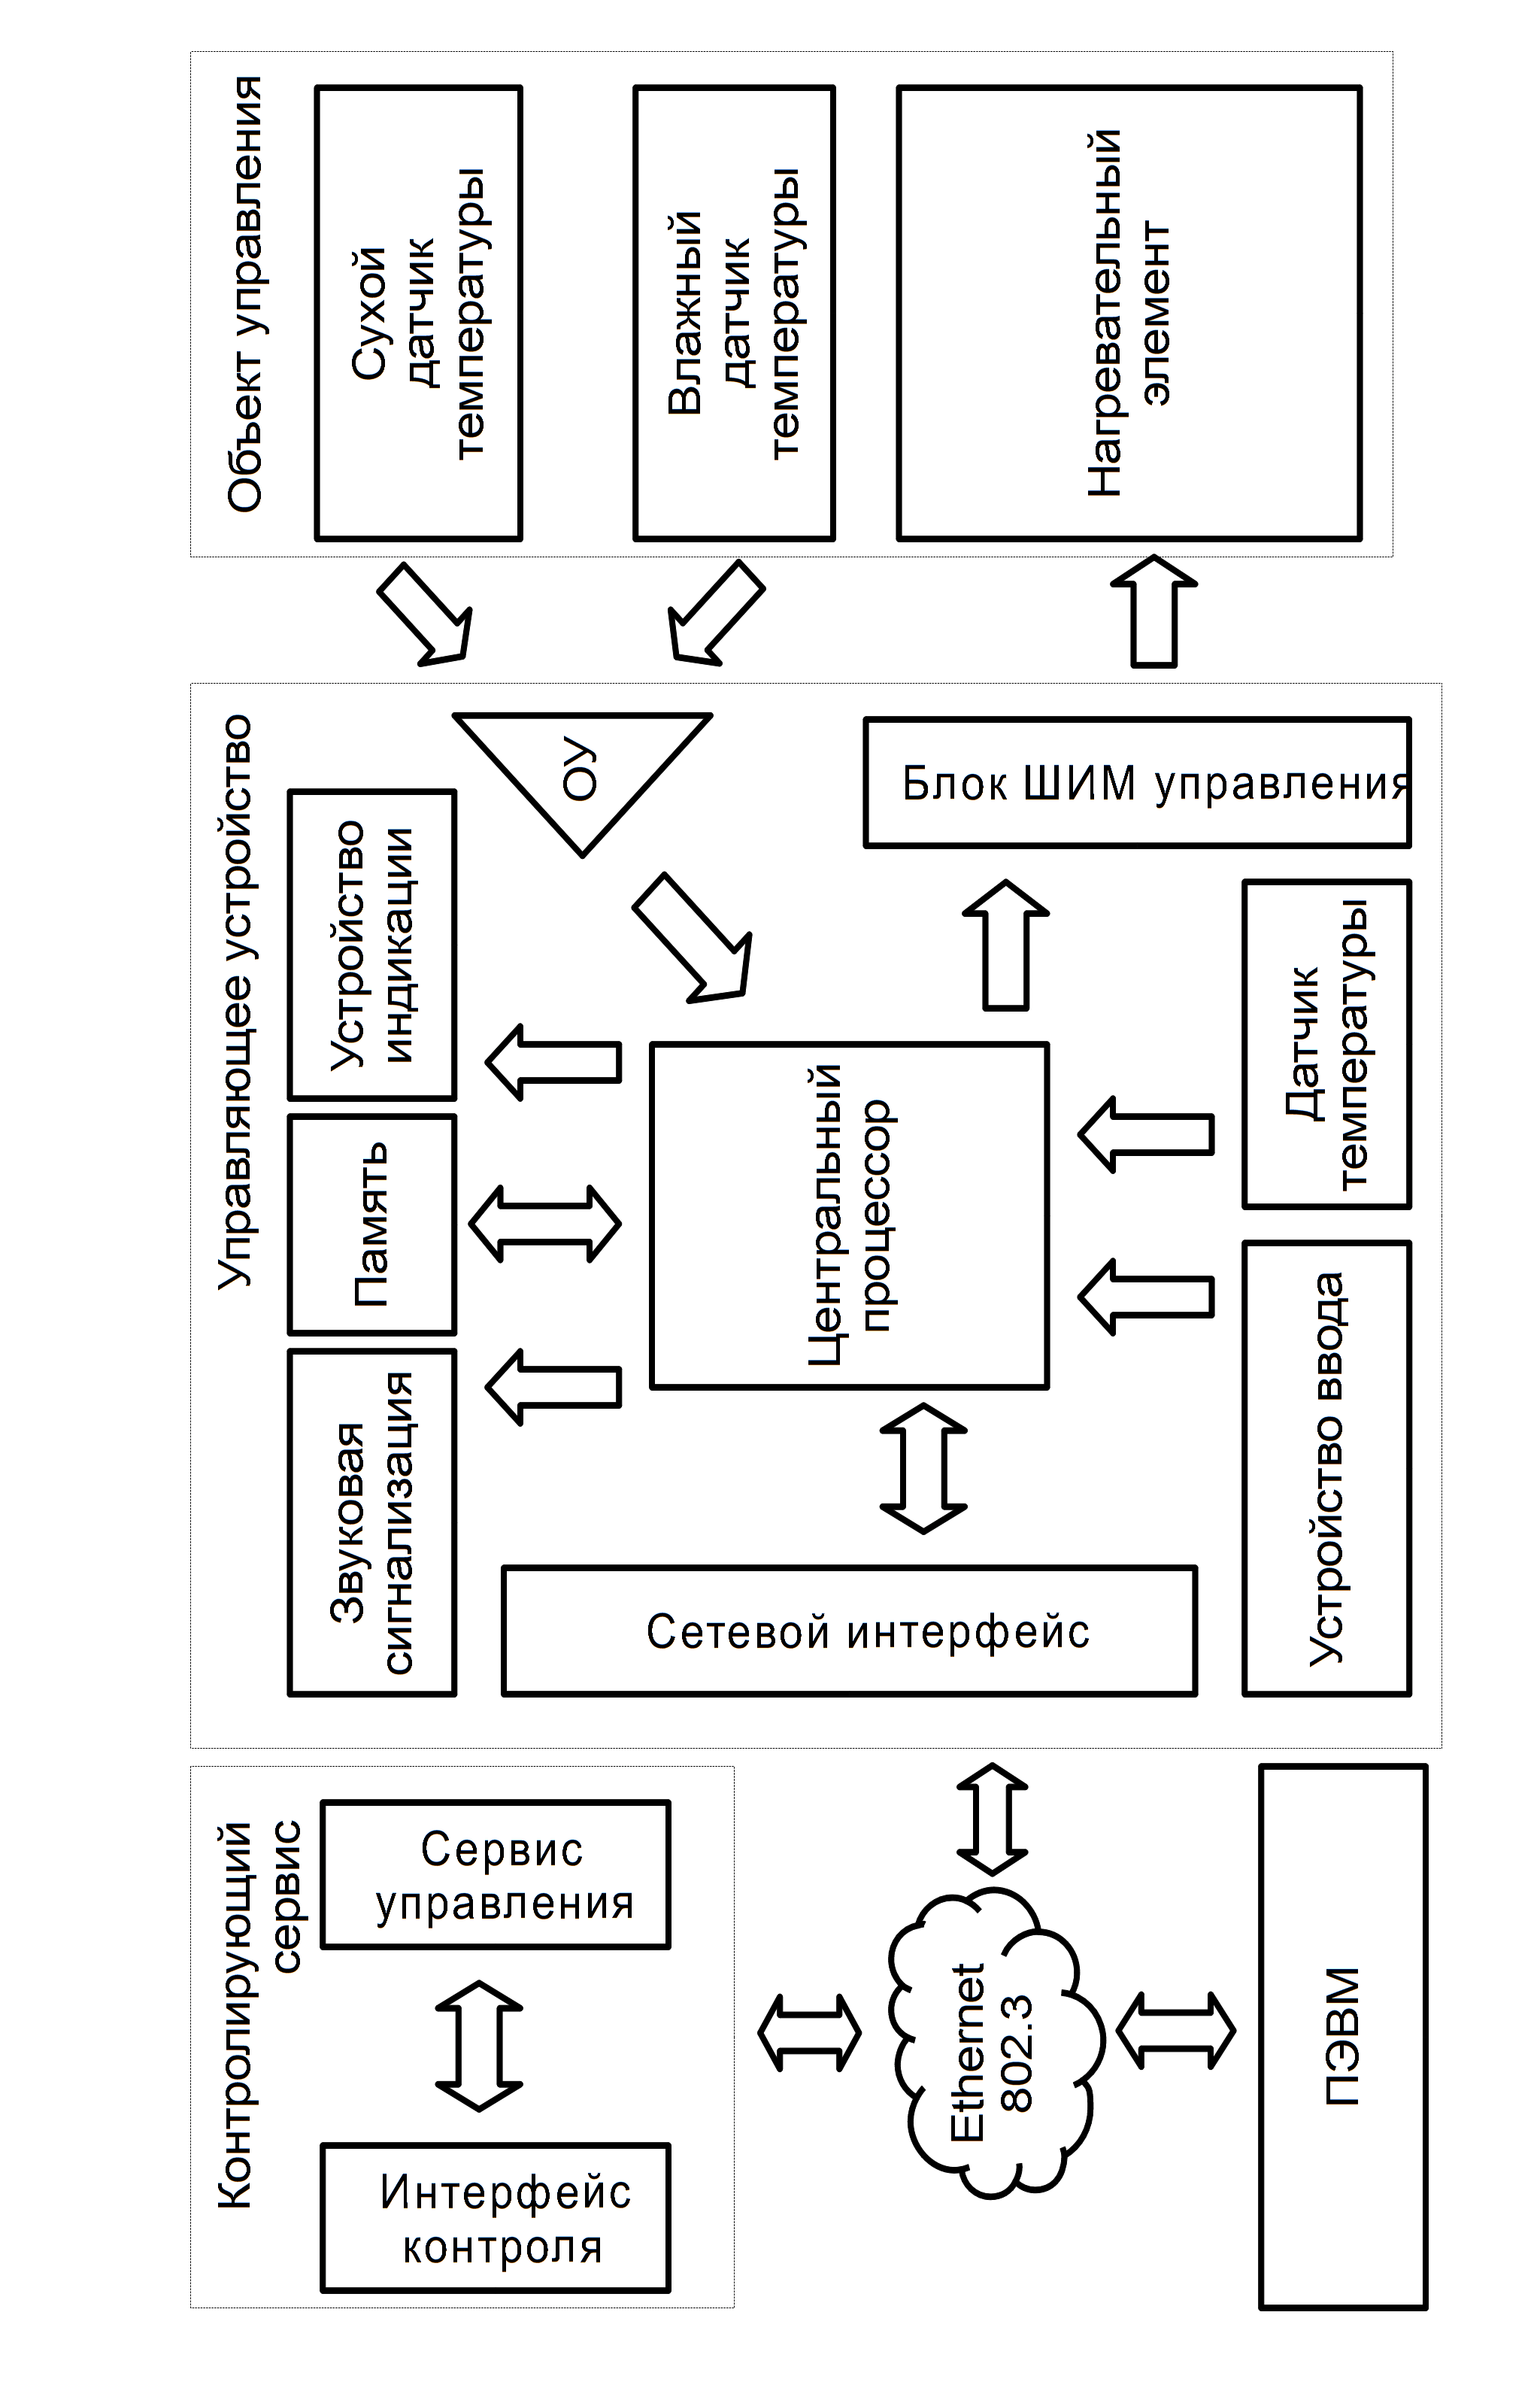
\includegraphics[bb=0 0 1500 2600, clip, scale=0.2]{struct_scheme.png}}
	%\caption{}
	%\label{img:structAdd}
\end{figure}
\newpage{}

\ESKDappendix{Обязательное}{Принципиальная электрическая схема управляющего устройства}
\begin{figure}[h]
	\center{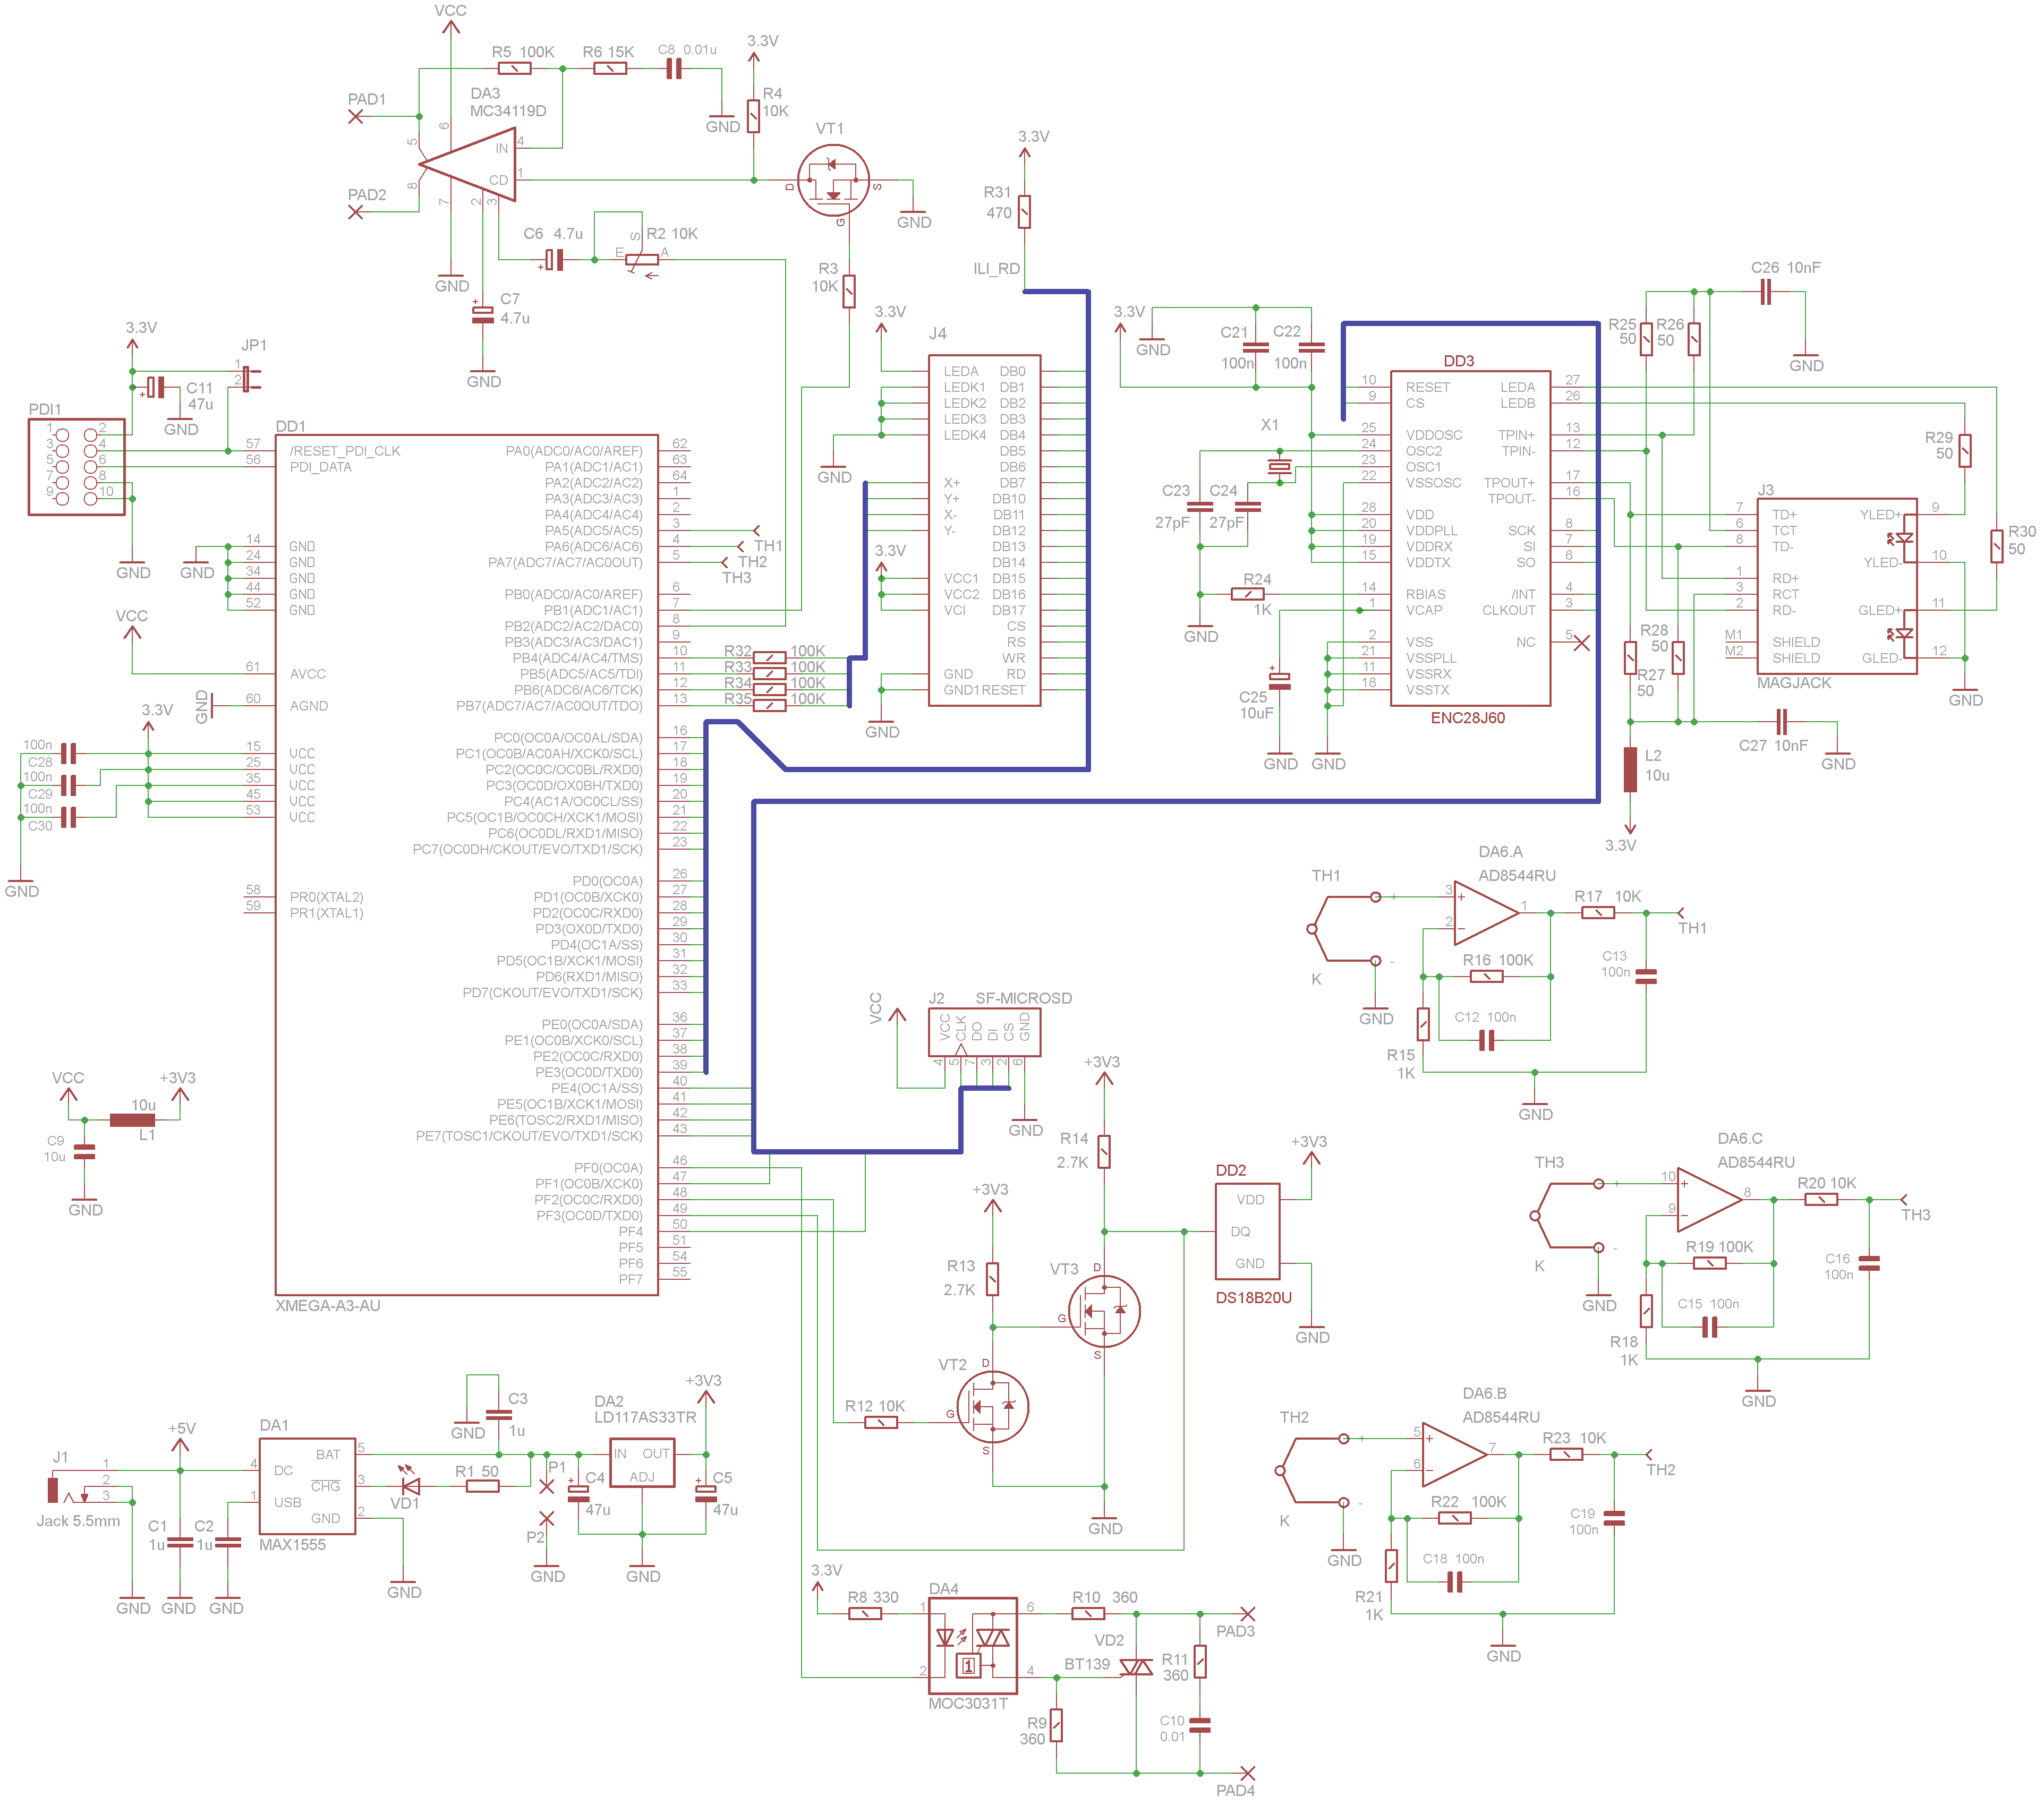
\includegraphics[bb=0 0 950 820, clip, scale=0.5]{scheme.png}}
	%\caption{}
	%\label{img:schemeAdd}
\end{figure}
\newpage{}

\ESKDappendix{Обязательное}{Топологическая схема управляющего устройства}
% \begin{figure}[h]
% 	\center{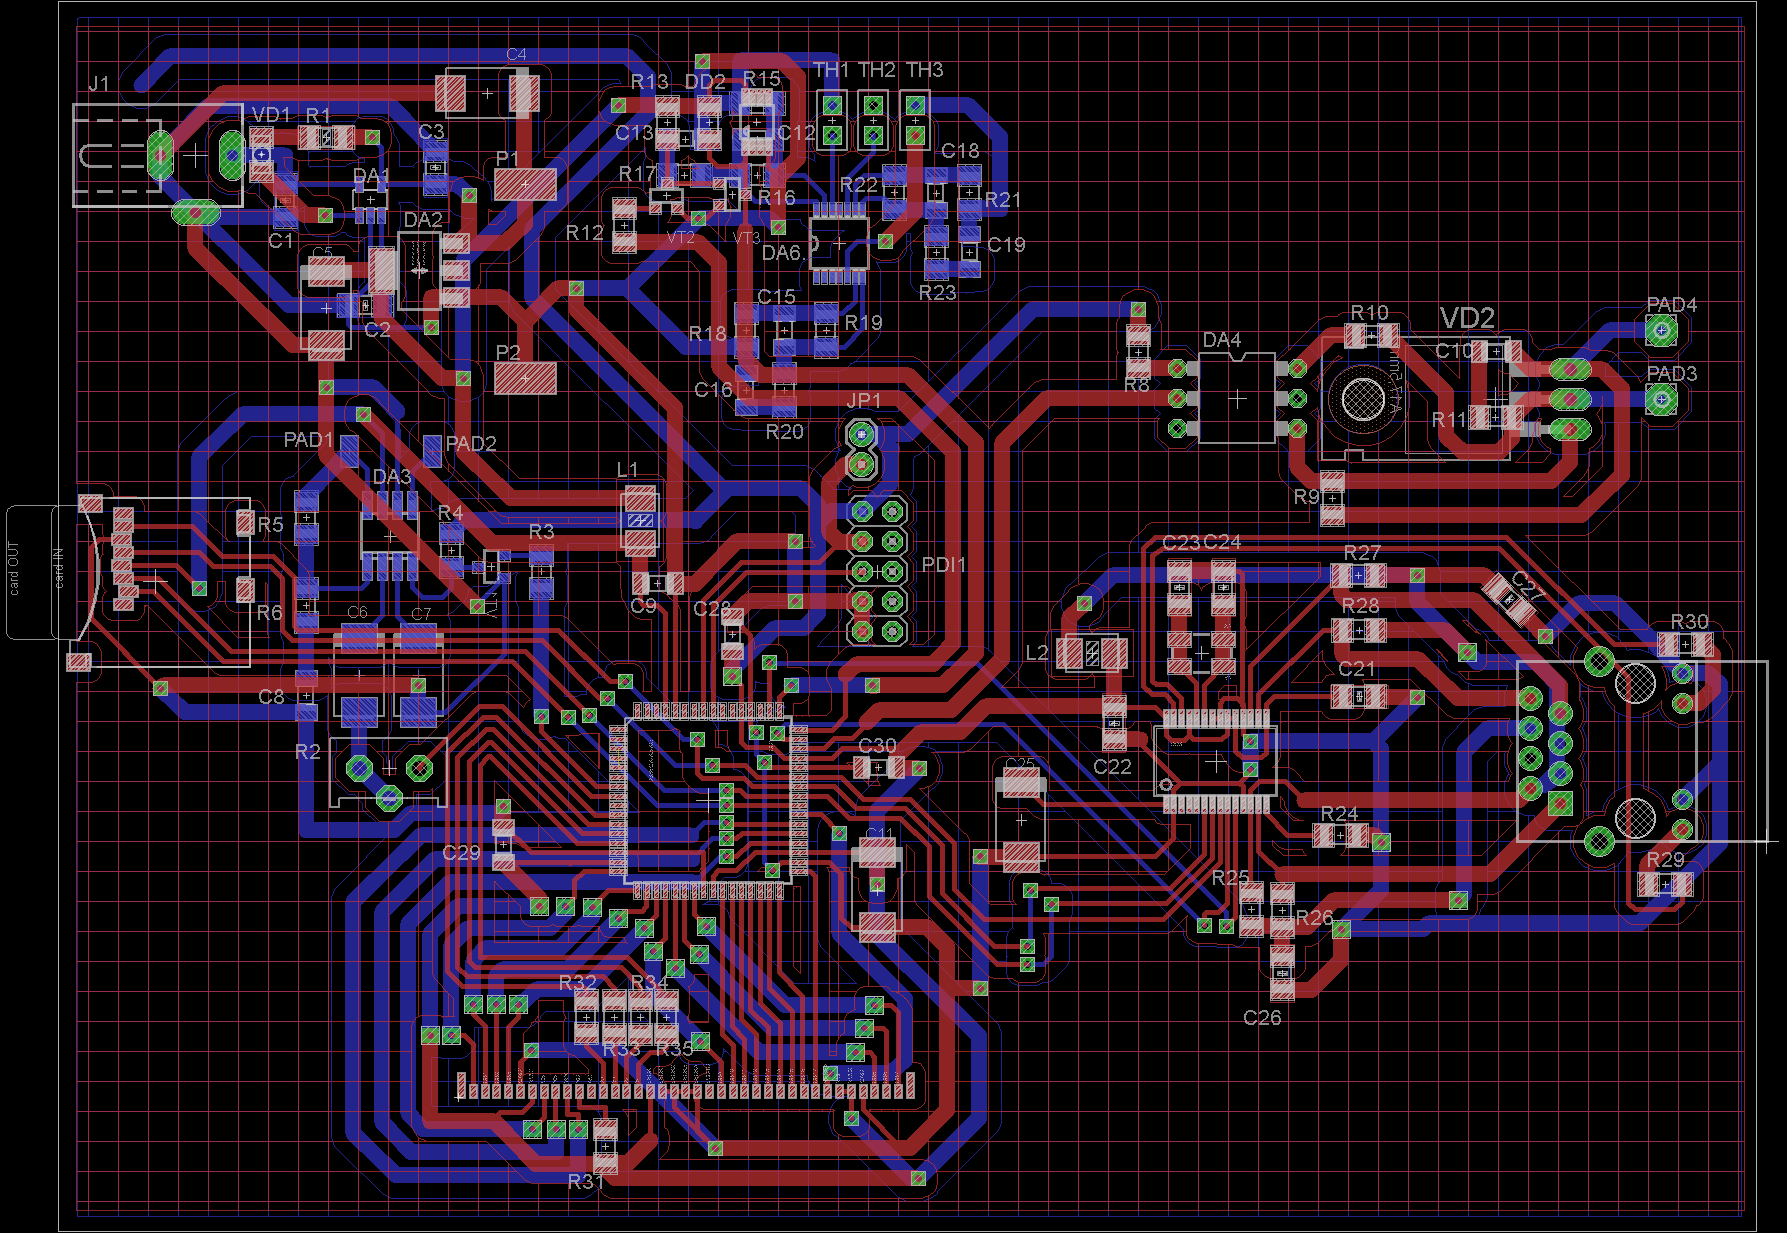
\includegraphics[bb=0 0 950 820, clip, scale=0.5]{pcb.png}}
% 	\caption{}
% 	\label{img:pcbAdd}
% \end{figure}
\newpage{}


\end{document}

